\chapter{Proposal for a new factorization of the fermionic determinant}
\label{chap:newfact}

The factorization procedure presented in the last chapter, accompanied by the factorization of fermionic observables, paved the way for the development of multi-level algorithms with dynamical fermions. Thanks to this technique, alongside the introduction of auxiliary multiboson fields, the quark determinant is factorized into terms which are local in the block fields, except for a small remainder, which depends on gauge fields defined across the whole lattice.
\\ In this work, we present a new factorization procedure for the fermionic determinant, based on the complete separation of the system dynamics in different regions, without the introduction of an overlapping region. Before we can actually apply this method to numerical simulations, we need to formalize the factorization of fermionic observables, which will be the next goal of our research and could be introduced naturally in this framework.
\\ Since the effectiveness of this factorization will be first tested on the Schwinger Model, we present the theoretical aspects of our proposal in the framework of this theory. Future simulations results will then be compared with the standard system described in Chapter 2 and 3, where no pre-conditioning was employed. 
\\ In the meanwhile, we offer a numerical confirmation of the validity of our proposal.

\section{Introduction}
We present here the theoretical framework for the factorization of the fermionic determinant. We will formalize this procedure for the massive Schwinger Model with two mass-degenerate quarks, whose description can be found in Chapter \ref{chap: HMC}. Recall that the action is given by a fermionic term and a gauge term:
\begin{equation}
    S = S_G + S_F
\end{equation}
but only the first one is relevant for the quark determinant factorization procedure. For commodity, we report its expression here:
\begin{equation}\label{S_Ferm}
\begin{split}
    S_F [\psi, \Bar{\psi}, U] &= (m_0 + 2) \sum_{n, \alpha} \Bar{\psi}_\alpha(n)\psi_\alpha(n) -  \\  
        & - \frac{1}{2}\sum_{\substack{n, \mu \\ \alpha, \beta}}\left[ \Bar{\psi}_\beta(n)(1 - \gamma_\mu)_{\beta, \alpha} U_\mu(n) \psi_\alpha(n + \hat{\mu}) + \Bar{\psi}_\beta (n+\hat{\mu}) (1 + \gamma_\mu)_{\beta, \alpha} U^\dagger_\mu(n) \psi_\alpha(n) \right] \\
\end{split}
\end{equation}
where $\gamma_\mu$ are the Dirac matrices shown in \eqref{gammas}, namely:
\begin{equation}
    \gamma_0 = - \sigma_3 = \begin{pmatrix}
 -1 & 0  \\
   0 & 1 \\
\end{pmatrix}
   \,\,\,\,\,\, \gamma_1 = \sigma_1 = \begin{pmatrix}
 0 & 1  \\
   1 & 0 \\
\end{pmatrix}
   \,\,\,\,\,\, \gamma_2 = i\gamma_0 \gamma_1 = \sigma_2 = \begin{pmatrix}
 0 & -i  \\
   i & 0 \\
\end{pmatrix}
\end{equation}
\\ Consider a lattice with spatial extent $L_1$ and with $2L_0$ time slices. For the space direction we will employ periodic boundary conditions, while for the time direction we will explore both open and periodic boundary conditions.
\\ The first step towards the factorization of the fermionic determinant consists in recasting the Dirac operator in a convenient sparse block matrix form. Fermions are represented by two-dimensional spinors, and it is useful to write them in terms of their chiral components with respect to $\gamma_0$:
\begin{equation}
    \psi(n) = \begin{pmatrix}
        \psi^+_n \\
        \psi^-_n
    \end{pmatrix} \hspace{10mm} \Bar{\psi}(n) = \begin{pmatrix}
        \Bar{\psi}^+_n \,\, \Bar{\psi}^-_n
    \end{pmatrix}
\end{equation}
It is also convenient to write gauge fields more compactly, hence we will make use of the identifications:
\begin{equation}
    U_\mu(n) = z_{n, n+\hat{\mu}} \hspace{10mm} U_\mu^\dagger (n) = \Bar{z}_{n, n + \hat{\mu}}
\end{equation}
From Eq. \eqref{S_Ferm} it is easy to see that we can write three different contributions to the action. 
The first contribution comes from the mass term:
\begin{equation}
    \Bar{m}_0 \left( \Bar{\psi}^+_n \psi^+_n + \Bar{\psi}^-_n \psi^-_n \right)
\end{equation}
which is diagonal in the chiral components of the quark fields. Then we have interactions in the space direction:
\begin{equation}
    - \left[ \Bar{\psi}(n) \left(1 - \gamma_1 \right) U_1(x) \psi(n + \hat{1}) + \Bar{\psi}(n + \hat{1}) \left(1 + \gamma_1 \right) U^\dagger_1(x) \psi(n) \right]
\end{equation}
\begin{figure}
    \centering


\tikzset{every picture/.style={line width=0.75pt}} %set default line width to 0.75pt        

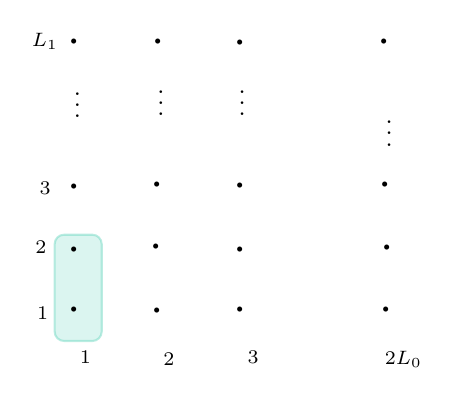
\begin{tikzpicture}[x=0.75pt,y=0.75pt,yscale=-1,xscale=1]
%uncomment if require: \path (0,300); %set diagram left start at 0, and has height of 300

%Rounded Rect [id:dp32613111558050933] 
\draw  [color={rgb, 255:red, 91; green, 210; blue, 185 }  ,draw opacity=0.41 ][fill={rgb, 255:red, 91; green, 210; blue, 185 }  ,fill opacity=0.22 ][line width=0.75]  (235.61,134.83) .. controls (235.61,132.33) and (237.64,130.3) .. (240.15,130.3) -- (253.75,130.3) .. controls (256.25,130.3) and (258.28,132.33) .. (258.28,134.83) -- (258.28,176.98) .. controls (258.28,179.48) and (256.25,181.51) .. (253.75,181.51) -- (240.15,181.51) .. controls (237.64,181.51) and (235.61,179.48) .. (235.61,176.98) -- cycle ;

% Text Node
\draw (240.42,31.05) node [anchor=north west][inner sep=0.75pt]  [font=\LARGE]  {$\cdot $};
% Text Node
\draw (243.37,52.51) node [anchor=north west][inner sep=0.75pt]  [font=\small]  {$\vdots $};
% Text Node
\draw (240.24,100.88) node [anchor=north west][inner sep=0.75pt]  [font=\LARGE]  {$\cdot $};
% Text Node
\draw (240.24,131.49) node [anchor=north west][inner sep=0.75pt]  [font=\LARGE]  {$\cdot $};
% Text Node
\draw (240.28,160.21) node [anchor=north west][inner sep=0.75pt]  [font=\LARGE]  {$\cdot $};
% Text Node
\draw (280.68,31.27) node [anchor=north west][inner sep=0.75pt]  [font=\LARGE]  {$\cdot $};
% Text Node
\draw (283.63,51.3) node [anchor=north west][inner sep=0.75pt]  [font=\small]  {$\vdots $};
% Text Node
\draw (280.36,100.29) node [anchor=north west][inner sep=0.75pt]  [font=\LARGE]  {$\cdot $};
% Text Node
\draw (279.76,130.1) node [anchor=north west][inner sep=0.75pt]  [font=\LARGE]  {$\cdot $};
% Text Node
\draw (280.11,160.87) node [anchor=north west][inner sep=0.75pt]  [font=\LARGE]  {$\cdot $};
% Text Node
\draw (320.17,31.67) node [anchor=north west][inner sep=0.75pt]  [font=\LARGE]  {$\cdot $};
% Text Node
\draw (322.72,51.5) node [anchor=north west][inner sep=0.75pt]  [font=\small]  {$\vdots $};
% Text Node
\draw (320.25,100.69) node [anchor=north west][inner sep=0.75pt]  [font=\LARGE]  {$\cdot $};
% Text Node
\draw (320.25,131.5) node [anchor=north west][inner sep=0.75pt]  [font=\LARGE]  {$\cdot $};
% Text Node
\draw (320.4,160.47) node [anchor=north west][inner sep=0.75pt]  [font=\LARGE]  {$\cdot $};
% Text Node
\draw (354.56,167.68) node [anchor=north west][inner sep=0.75pt]  [font=\small]  {$\dotsc $};
% Text Node
\draw (354.63,137.09) node [anchor=north west][inner sep=0.75pt]  [font=\small]  {$\dotsc $};
% Text Node
\draw (355.03,107.72) node [anchor=north west][inner sep=0.75pt]  [font=\small]  {$\dotsc $};
% Text Node
\draw (355.13,38.18) node [anchor=north west][inner sep=0.75pt]  [font=\small]  {$\dotsc $};
% Text Node
\draw (389.61,31.23) node [anchor=north west][inner sep=0.75pt]  [font=\LARGE]  {$\cdot $};
% Text Node
\draw (393.57,66.1) node [anchor=north west][inner sep=0.75pt]  [font=\small]  {$\vdots $};
% Text Node
\draw (390.23,100.27) node [anchor=north west][inner sep=0.75pt]  [font=\LARGE]  {$\cdot $};
% Text Node
\draw (391.23,130.48) node [anchor=north west][inner sep=0.75pt]  [font=\LARGE]  {$\cdot $};
% Text Node
\draw (390.85,160.43) node [anchor=north west][inner sep=0.75pt]  [font=\LARGE]  {$\cdot $};
% Text Node
\draw (246.25,184.84) node [anchor=north west][inner sep=0.75pt]  [font=\scriptsize]  {$1$};
% Text Node
\draw (286.45,185.75) node [anchor=north west][inner sep=0.75pt]  [font=\scriptsize]  {$2$};
% Text Node
\draw (327.04,184.77) node [anchor=north west][inner sep=0.75pt]  [font=\scriptsize]  {$3$};
% Text Node
\draw (393.19,184.87) node [anchor=north west][inner sep=0.75pt]  [font=\scriptsize]  {$2L_{0}$};
% Text Node
\draw (225.64,163.65) node [anchor=north west][inner sep=0.75pt]  [font=\scriptsize]  {$1$};
% Text Node
\draw (224.8,131.69) node [anchor=north west][inner sep=0.75pt]  [font=\scriptsize]  {$2$};
% Text Node
\draw (226.91,103.5) node [anchor=north west][inner sep=0.75pt]  [font=\scriptsize]  {$3$};
% Text Node
\draw (223.11,31.79) node [anchor=north west][inner sep=0.75pt]  [font=\scriptsize]  {$L_{1}$};


\end{tikzpicture}


    \caption{Visualization of the interaction along the space direction between two points of the first time slice.}
    \label{fig: space int}
\end{figure}
Consider for instance the interaction between the sites $1$ and $2$ on the first time slice (see Figure \eqref{fig: space int}), its expression is given by:
\begin{equation}
    - \left[ \begin{pmatrix}
        \Bar{\psi}^+_1 \,\, \Bar{\psi}^-_1
    \end{pmatrix} z_{1,2} (1 - \gamma_1) \begin{pmatrix}
        \psi^+_2 \\
        \psi^-_2
    \end{pmatrix} + \begin{pmatrix}
        \Bar{\psi}^+_2 \,\, \Bar{\psi}^-_2
    \end{pmatrix} \Bar{z}_{1,2} (1 + \gamma_1) \begin{pmatrix}
        \psi^+_1 \\
        \psi^-_1
    \end{pmatrix} \right]
\end{equation}
and using the explicit expression for $(1 \pm \gamma_1)$, it becomes:
\begin{equation}
    - z_{1,2} \left[ \Bar{\psi}^+_1 \psi_2^+ - \Bar{\psi}^+_1 \psi_2^- - \Bar{\psi}_1^-\psi_2^+ + \Bar{\psi}_1^- \psi_2^- \right] - \Bar{z}_{1,2} \left[ \Bar{\psi}^+_2 \psi_1^+ - \Bar{\psi}^+_2 \psi_1^- - \Bar{\psi}_2^-\psi_1^+ + \Bar{\psi}_2^- \psi_1^- \right]
\end{equation}
and for other pairs of sites we get analogous contributions. The mass term and the spatial interaction for the lattice sites lying on the first time slice can then be written compactly in a matrix form. Indeed, if we define:
\begin{equation}
    X_1 = \frac{1}{2} \begin{pmatrix}
        2 \Bar{m}_0 & - z_{1,2} & 0 & \dots & & 0 & - \Bar{z}_{L_1, 1} \\
        - \Bar{z}_{1,2} & 2 \Bar{m}_0 & - z_{2,3} & 0 & \dots & & 0 \\
        0 & - \Bar{z}_{2,3} & 2 \Bar{m}_0 & - z_{3,4} & 0 & \dots & \vdots \\
        \\
        \vdots & & & \ddots \\
        \\
        \\
        & & & & & & 0 \\
        0 & & & & - \Bar{z}_{L_1 - 2, L_1 - 1} & 2 \Bar{m}_0 & - z_{L_1 - 1, L_1} \\
        - z_{L_1, 1} & 0 & \dots & & 0 & - \Bar{z}_{L_1 - 1, L_1} & 2 \Bar{m}_0 \\ 
    \end{pmatrix}
\end{equation}
for which it holds $X_1 = X_1^{\dagger}$, i.e. it is hermitian, and:
\begin{equation}
    Y_1 = \frac{1}{2} \begin{pmatrix}
        0 & z_{1,2} & 0 & \dots & & 0 & - \Bar{z}_{L_1, 1} \\
        - \Bar{z}_{1,2} & 0 & z_{2,3} & 0 & \dots & & 0 \\
        0 & - \Bar{z}_{2,3} & 0 & - z_{3,4} & 0 & \dots & \vdots \\
        \\
        \vdots & & & \ddots \\
        \\
        \\
        & & & & & & 0 \\
        0 & & & & - \Bar{z}_{L_1 - 2, L_1 - 1} & 0 & - z_{L_1 - 1, L_1} \\
        - z_{L_1, 1} & 0 & \dots & & 0 & - \Bar{z}_{L_1 - 1, L_1} & 0 \\ 
    \end{pmatrix}
\end{equation}
which is an anti-hermitian matrix $Y_1 = - Y_1^\dagger$, then we can write the mass and spatial contribution to the Dirac operator for the first time slice as:
\begin{equation}
    D_1 = \begin{pmatrix}
        X_1 & Y_1 \\
        Y_1 & X_1 \\
    \end{pmatrix}
\end{equation}
and similarly for all the other time slices.
\begin{figure}
    \centering


\tikzset{every picture/.style={line width=0.75pt}} %set default line width to 0.75pt        

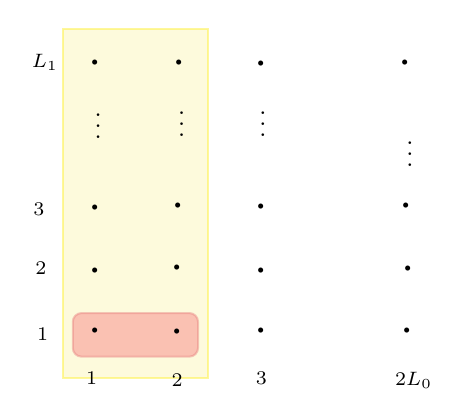
\begin{tikzpicture}[x=0.75pt,y=0.75pt,yscale=-1,xscale=1]
%uncomment if require: \path (0,300); %set diagram left start at 0, and has height of 300

%Shape: Rectangle [id:dp05909713682911022] 
\draw  [color={rgb, 255:red, 253; green, 239; blue, 52 }  ,draw opacity=0.49 ][fill={rgb, 255:red, 247; green, 235; blue, 109 }  ,fill opacity=0.24 ] (229.69,20.94) -- (299.36,20.94) -- (299.36,189.28) -- (229.69,189.28) -- cycle ;
%Rounded Rect [id:dp5474542337645614] 
\draw  [color={rgb, 255:red, 229; green, 124; blue, 125 }  ,draw opacity=0.41 ][fill={rgb, 255:red, 247; green, 134; blue, 134 }  ,fill opacity=0.49 ] (234.36,162.14) .. controls (234.36,159.82) and (236.24,157.94) .. (238.56,157.94) -- (290.49,157.94) .. controls (292.81,157.94) and (294.69,159.82) .. (294.69,162.14) -- (294.69,174.74) .. controls (294.69,177.06) and (292.81,178.94) .. (290.49,178.94) -- (238.56,178.94) .. controls (236.24,178.94) and (234.36,177.06) .. (234.36,174.74) -- cycle ;

% Text Node
\draw (240.42,31.05) node [anchor=north west][inner sep=0.75pt]  [font=\LARGE]  {$\cdot $};
% Text Node
\draw (243.37,52.51) node [anchor=north west][inner sep=0.75pt]  [font=\small]  {$\vdots $};
% Text Node
\draw (240.24,101.21) node [anchor=north west][inner sep=0.75pt]  [font=\LARGE]  {$\cdot $};
% Text Node
\draw (240.24,131.49) node [anchor=north west][inner sep=0.75pt]  [font=\LARGE]  {$\cdot $};
% Text Node
\draw (240.28,160.21) node [anchor=north west][inner sep=0.75pt]  [font=\LARGE]  {$\cdot $};
% Text Node
\draw (280.68,31.27) node [anchor=north west][inner sep=0.75pt]  [font=\LARGE]  {$\cdot $};
% Text Node
\draw (283.63,51.3) node [anchor=north west][inner sep=0.75pt]  [font=\small]  {$\vdots $};
% Text Node
\draw (280.36,100.29) node [anchor=north west][inner sep=0.75pt]  [font=\LARGE]  {$\cdot $};
% Text Node
\draw (279.76,130.1) node [anchor=north west][inner sep=0.75pt]  [font=\LARGE]  {$\cdot $};
% Text Node
\draw (280.11,160.87) node [anchor=north west][inner sep=0.75pt]  [font=\LARGE]  {$\cdot $};
% Text Node
\draw (320.17,31.67) node [anchor=north west][inner sep=0.75pt]  [font=\LARGE]  {$\cdot $};
% Text Node
\draw (322.72,51.5) node [anchor=north west][inner sep=0.75pt]  [font=\small]  {$\vdots $};
% Text Node
\draw (320.25,100.69) node [anchor=north west][inner sep=0.75pt]  [font=\LARGE]  {$\cdot $};
% Text Node
\draw (320.25,131.5) node [anchor=north west][inner sep=0.75pt]  [font=\LARGE]  {$\cdot $};
% Text Node
\draw (320.4,160.47) node [anchor=north west][inner sep=0.75pt]  [font=\LARGE]  {$\cdot $};
% Text Node
\draw (354.56,167.68) node [anchor=north west][inner sep=0.75pt]  [font=\small]  {$\dotsc $};
% Text Node
\draw (354.63,137.09) node [anchor=north west][inner sep=0.75pt]  [font=\small]  {$\dotsc $};
% Text Node
\draw (355.03,107.72) node [anchor=north west][inner sep=0.75pt]  [font=\small]  {$\dotsc $};
% Text Node
\draw (355.13,38.18) node [anchor=north west][inner sep=0.75pt]  [font=\small]  {$\dotsc $};
% Text Node
\draw (389.61,31.23) node [anchor=north west][inner sep=0.75pt]  [font=\LARGE]  {$\cdot $};
% Text Node
\draw (393.57,66.1) node [anchor=north west][inner sep=0.75pt]  [font=\small]  {$\vdots $};
% Text Node
\draw (390.23,100.27) node [anchor=north west][inner sep=0.75pt]  [font=\LARGE]  {$\cdot $};
% Text Node
\draw (391.23,130.48) node [anchor=north west][inner sep=0.75pt]  [font=\LARGE]  {$\cdot $};
% Text Node
\draw (390.85,160.43) node [anchor=north west][inner sep=0.75pt]  [font=\LARGE]  {$\cdot $};
% Text Node
\draw (239.25,184.84) node [anchor=north west][inner sep=0.75pt]  [font=\scriptsize]  {$1$};
% Text Node
\draw (280.45,185.75) node [anchor=north west][inner sep=0.75pt]  [font=\scriptsize]  {$2$};
% Text Node
\draw (321.04,184.77) node [anchor=north west][inner sep=0.75pt]  [font=\scriptsize]  {$3$};
% Text Node
\draw (388.19,184.87) node [anchor=north west][inner sep=0.75pt]  [font=\scriptsize]  {$2L_{0}$};
% Text Node
\draw (215.64,163.65) node [anchor=north west][inner sep=0.75pt]  [font=\scriptsize]  {$1$};
% Text Node
\draw (214.8,131.69) node [anchor=north west][inner sep=0.75pt]  [font=\scriptsize]  {$2$};
% Text Node
\draw (213.91,103.5) node [anchor=north west][inner sep=0.75pt]  [font=\scriptsize]  {$3$};
% Text Node
\draw (213.11,31.79) node [anchor=north west][inner sep=0.75pt]  [font=\scriptsize]  {$L_{1}$};


\end{tikzpicture}

    \caption{Visualization of the interaction along the time direction between $1$ and $L_1 + 1$, the first sites of the time slices 1 and 2, i.e. Eq. \eqref{time inter}.}
    \label{fig: time int}
\end{figure}
\\ The last contribution we should consider comes from interactions in the time direction, for instance:
\begin{equation}
    - \left[ \Bar{\psi}(n) \left(1 - \gamma_0 \right) U_0(x) \psi(n + \hat{0}) + \Bar{\psi}(n + \hat{0}) \left(1 + \gamma_0 \right) U^\dagger_0(x) \psi(n) \right]
\end{equation}
and analogously to what we have done for spatial contributions, we can write the interaction between two points $1$ and $L_1 + 1$ explicitly as (see Fig. \eqref{fig: time int}):
\begin{equation}\label{time inter}
    \begin{split}
        &- 2 \left[ \begin{pmatrix}
        \Bar{\psi}^+_1 \,\, \Bar{\psi}^-_1
    \end{pmatrix} z_{1,L_1 + 1} (1 - \gamma_0) \begin{pmatrix}
        \psi^+_{L_1 + 1} \\
        \psi^-_{L_1 + 1}
    \end{pmatrix} + \begin{pmatrix}
        \Bar{\psi}^+_{L_1 + 1} \,\, \Bar{\psi}^-_{L_1 + 1}
    \end{pmatrix} \Bar{z}_{1,L_1 + 1} (1 + \gamma_0) \begin{pmatrix}
        \psi^+_1 \\
        \psi^-_1
    \end{pmatrix} \right] = \\
   & = -2 \left[ z_{1, L_1 + 1} \Bar{\psi}_1^+ \psi_{L_1 + 1}^+ + \Bar{z}_{1, L_1 + 1} \Bar{\psi}_{L_1 + 1}^- \psi_1^- \right]
    \end{split}
\end{equation}
Notice that these contributions are diagonal in the chiral components. We can thus define the matrix:
\begin{equation}
    \Lambda_{1, L_1 + 1} = - \begin{pmatrix}
        z_{1, L_1 + 1} & 0 & \dots &  & & 0  \\
        0 & z_{2, L_1 + 2} & 0 & \dots &  & \vdots \\
        \vdots & 0 & \ddots & 0 \\
        \\
        & & & & &  0 \\
        0 & & & \dots & 0 & z_{L_1, 2L_1} \\ 
    \end{pmatrix} = \Lambda^{T}_{1, L_1 + 1}
\end{equation}
and consequently the contributions to the Dirac operator coming from interactions along the time direction between the first two time slices can be expressed with the following matrices:
\begin{equation} \label{time interaction matrix}
    D_{1, L_1 + 1} = \begin{pmatrix}
        \Lambda_{1, L_1 + 1} & \mathbb{0} \\
        \mathbb{0} & \mathbb{0} \\
    \end{pmatrix} \hspace{10mm} \Tilde{D}_{1, L_1 + 1} = \begin{pmatrix}
        \mathbb{0} & \mathbb{0} \\
        \mathbb{0} & \Bar{\Lambda}_{1, L_1 + 1} \\
    \end{pmatrix}
\end{equation}
and analogously for the other time slices\footnote{Notice that in the following sections $\mathbb{0}$ typically represents a $L_1 \cross L_1$ block of zeros, unless otherwise stated, but in any case its dimensions should be clear from the context. For instance, in definition \eqref{D matrix} it has dimensions $2L_1 \cross 2L_1.$}. 
\\ Taking into account all the contributions, we can write the Dirac operator as:
\begin{equation}\label{D matrix}
    \mathcal{D} = \begin{pmatrix}
        D_1 & D_{1,2} & \mathbb{0} & \dots &  & \Tilde{J}  \\
        \Tilde{D}_{1,2} & D_2 & D_{2,3} & \mathbb{0} & \dots & \mathbb{0} \\
        \mathbb{0} & \Tilde{D}_{2,3} & D_3 & D_{3,4} & \mathbb{0} & \vdots \\
        \vdots & & & \ddots & \\
        \\
        \mathbb{0} & & & & D_{2L_0 - 1} & D_{2L_0 - 1, 2L_0} \\
        J & \mathbb{0} & \dots & \mathbb{0} & \Tilde{D}_{2L_0 - 1, 2L_0} & D_{2L_0} \\ 
    \end{pmatrix}
\end{equation}
where:
\begin{equation}
    J = \left\{ \begin{array}{rcl} \mathbb{0} \hspace{10mm} \mbox{open boundary conditions}& \\ D_{L_0, 1}  \hspace{3mm} \mbox{periodic boundary conditions}&  \\ \end{array} \right.
\end{equation}
The expression \eqref{D matrix} for the Dirac operator allows us to write the fermion action in a quadratic form, hence when we integrate out the Grassmann variables in the path integral we get:
\begin{equation}
    \int \mathcal{D}[\psi] \mathcal{D}[\Bar{\psi}] e^{-\Bar{\psi} \mathcal{D} \psi} = \det(\mathcal{D})
\end{equation}

\section{Open boundary conditions}\label{OpenBC}
\begin{figure}
    \centering
\tikzset{every picture/.style={line width=0.75pt}} %set default line width to 0.75pt        
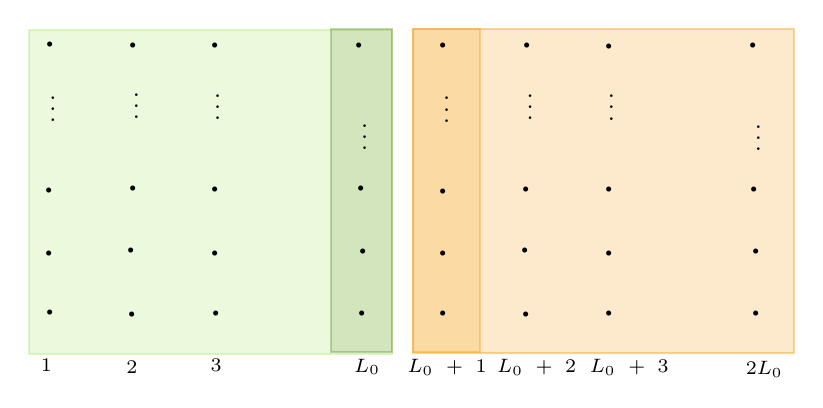
\begin{tikzpicture}[x=0.75pt,y=0.75pt,yscale=-1,xscale=1]
%uncomment if require: \path (0,300); %set diagram left start at 0, and has height of 300

%Shape: Rectangle [id:dp3848625804971728] 
\draw  [color={rgb, 255:red, 184; green, 233; blue, 134 }  ,draw opacity=0.46 ][fill={rgb, 255:red, 184; green, 233; blue, 134 }  ,fill opacity=0.28 ] (234.89,30) -- (410.03,30) -- (410.03,185.94) -- (234.89,185.94) -- cycle ;
%Shape: Rectangle [id:dp9450776254434018] 
\draw  [color={rgb, 255:red, 65; green, 117; blue, 5 }  ,draw opacity=0.29 ][fill={rgb, 255:red, 65; green, 117; blue, 5 }  ,fill opacity=0.15 ] (380.36,29.33) -- (410.03,29.33) -- (410.03,185.28) -- (380.36,185.28) -- cycle ;
%Shape: Rectangle [id:dp43101617233074474] 
\draw  [color={rgb, 255:red, 245; green, 166; blue, 35 }  ,draw opacity=0.47 ][fill={rgb, 255:red, 245; green, 166; blue, 35 }  ,fill opacity=0.23 ] (419.89,29.67) -- (603.69,29.67) -- (603.69,185.61) -- (419.89,185.61) -- cycle ;
%Shape: Rectangle [id:dp31365082950207435] 
\draw  [color={rgb, 255:red, 245; green, 166; blue, 35 }  ,draw opacity=0.46 ][fill={rgb, 255:red, 245; green, 166; blue, 35 }  ,fill opacity=0.24 ] (419.89,29.67) -- (452.36,29.67) -- (452.36,185.28) -- (419.89,185.28) -- cycle ;

% Text Node
\draw (240.42,31.05) node [anchor=north west][inner sep=0.75pt]  [font=\LARGE]  {$\cdot $};
% Text Node
\draw (243.37,52.51) node [anchor=north west][inner sep=0.75pt]  [font=\small]  {$\vdots $};
% Text Node
\draw (240.24,101.21) node [anchor=north west][inner sep=0.75pt]  [font=\LARGE]  {$\cdot $};
% Text Node
\draw (240.24,131.49) node [anchor=north west][inner sep=0.75pt]  [font=\LARGE]  {$\cdot $};
% Text Node
\draw (240.28,160.21) node [anchor=north west][inner sep=0.75pt]  [font=\LARGE]  {$\cdot $};
% Text Node
\draw (280.68,31.27) node [anchor=north west][inner sep=0.75pt]  [font=\LARGE]  {$\cdot $};
% Text Node
\draw (283.63,51.3) node [anchor=north west][inner sep=0.75pt]  [font=\small]  {$\vdots $};
% Text Node
\draw (280.36,100.29) node [anchor=north west][inner sep=0.75pt]  [font=\LARGE]  {$\cdot $};
% Text Node
\draw (279.76,130.1) node [anchor=north west][inner sep=0.75pt]  [font=\LARGE]  {$\cdot $};
% Text Node
\draw (280.11,160.87) node [anchor=north west][inner sep=0.75pt]  [font=\LARGE]  {$\cdot $};
% Text Node
\draw (320.17,31.67) node [anchor=north west][inner sep=0.75pt]  [font=\LARGE]  {$\cdot $};
% Text Node
\draw (322.72,51.5) node [anchor=north west][inner sep=0.75pt]  [font=\small]  {$\vdots $};
% Text Node
\draw (320.25,100.69) node [anchor=north west][inner sep=0.75pt]  [font=\LARGE]  {$\cdot $};
% Text Node
\draw (320.25,131.5) node [anchor=north west][inner sep=0.75pt]  [font=\LARGE]  {$\cdot $};
% Text Node
\draw (320.4,160.47) node [anchor=north west][inner sep=0.75pt]  [font=\LARGE]  {$\cdot $};
% Text Node
\draw (354.56,167.68) node [anchor=north west][inner sep=0.75pt]  [font=\small]  {$\dotsc $};
% Text Node
\draw (354.63,137.09) node [anchor=north west][inner sep=0.75pt]  [font=\small]  {$\dotsc $};
% Text Node
\draw (355.03,107.72) node [anchor=north west][inner sep=0.75pt]  [font=\small]  {$\dotsc $};
% Text Node
\draw (355.13,38.18) node [anchor=north west][inner sep=0.75pt]  [font=\small]  {$\dotsc $};
% Text Node
\draw (389.61,31.23) node [anchor=north west][inner sep=0.75pt]  [font=\LARGE]  {$\cdot $};
% Text Node
\draw (393.57,66.1) node [anchor=north west][inner sep=0.75pt]  [font=\small]  {$\vdots $};
% Text Node
\draw (390.23,100.27) node [anchor=north west][inner sep=0.75pt]  [font=\LARGE]  {$\cdot $};
% Text Node
\draw (391.23,130.48) node [anchor=north west][inner sep=0.75pt]  [font=\LARGE]  {$\cdot $};
% Text Node
\draw (390.85,160.43) node [anchor=north west][inner sep=0.75pt]  [font=\LARGE]  {$\cdot $};
% Text Node
\draw (239.25,186.84) node [anchor=north west][inner sep=0.75pt]  [font=\scriptsize]  {$1$};
% Text Node
\draw (280.45,187.75) node [anchor=north west][inner sep=0.75pt]  [font=\scriptsize]  {$2$};
% Text Node
\draw (321.04,186.77) node [anchor=north west][inner sep=0.75pt]  [font=\scriptsize]  {$3$};
% Text Node
\draw (390.19,186.87) node [anchor=north west][inner sep=0.75pt]  [font=\scriptsize]  {$L_{0}$};
% Text Node
\draw (430.09,31.4) node [anchor=north west][inner sep=0.75pt]  [font=\LARGE]  {$\cdot $};
% Text Node
\draw (433.03,52.87) node [anchor=north west][inner sep=0.75pt]  [font=\small]  {$\vdots $};
% Text Node
\draw (429.91,101.57) node [anchor=north west][inner sep=0.75pt]  [font=\LARGE]  {$\cdot $};
% Text Node
\draw (429.91,131.85) node [anchor=north west][inner sep=0.75pt]  [font=\LARGE]  {$\cdot $};
% Text Node
\draw (429.95,160.56) node [anchor=north west][inner sep=0.75pt]  [font=\LARGE]  {$\cdot $};
% Text Node
\draw (470.35,31.62) node [anchor=north west][inner sep=0.75pt]  [font=\LARGE]  {$\cdot $};
% Text Node
\draw (473.3,51.65) node [anchor=north west][inner sep=0.75pt]  [font=\small]  {$\vdots $};
% Text Node
\draw (470.03,100.65) node [anchor=north west][inner sep=0.75pt]  [font=\LARGE]  {$\cdot $};
% Text Node
\draw (469.43,130.45) node [anchor=north west][inner sep=0.75pt]  [font=\LARGE]  {$\cdot $};
% Text Node
\draw (469.78,161.22) node [anchor=north west][inner sep=0.75pt]  [font=\LARGE]  {$\cdot $};
% Text Node
\draw (509.83,32.02) node [anchor=north west][inner sep=0.75pt]  [font=\LARGE]  {$\cdot $};
% Text Node
\draw (512.38,51.85) node [anchor=north west][inner sep=0.75pt]  [font=\small]  {$\vdots $};
% Text Node
\draw (509.91,101.05) node [anchor=north west][inner sep=0.75pt]  [font=\LARGE]  {$\cdot $};
% Text Node
\draw (509.91,131.85) node [anchor=north west][inner sep=0.75pt]  [font=\LARGE]  {$\cdot $};
% Text Node
\draw (510.07,160.82) node [anchor=north west][inner sep=0.75pt]  [font=\LARGE]  {$\cdot $};
% Text Node
\draw (544.23,168.03) node [anchor=north west][inner sep=0.75pt]  [font=\small]  {$\dotsc $};
% Text Node
\draw (544.3,137.45) node [anchor=north west][inner sep=0.75pt]  [font=\small]  {$\dotsc $};
% Text Node
\draw (544.7,108.08) node [anchor=north west][inner sep=0.75pt]  [font=\small]  {$\dotsc $};
% Text Node
\draw (544.79,38.53) node [anchor=north west][inner sep=0.75pt]  [font=\small]  {$\dotsc $};
% Text Node
\draw (579.28,31.58) node [anchor=north west][inner sep=0.75pt]  [font=\LARGE]  {$\cdot $};
% Text Node
\draw (583.24,66.45) node [anchor=north west][inner sep=0.75pt]  [font=\small]  {$\vdots $};
% Text Node
\draw (579.9,100.62) node [anchor=north west][inner sep=0.75pt]  [font=\LARGE]  {$\cdot $};
% Text Node
\draw (580.9,130.83) node [anchor=north west][inner sep=0.75pt]  [font=\LARGE]  {$\cdot $};
% Text Node
\draw (580.52,160.78) node [anchor=north west][inner sep=0.75pt]  [font=\LARGE]  {$\cdot $};
% Text Node
\draw (415.92,187.2) node [anchor=north west][inner sep=0.75pt]  [font=\scriptsize]  {$L_{0} \ +\ 1$};
% Text Node
\draw (459.11,187.1) node [anchor=north west][inner sep=0.75pt]  [font=\scriptsize]  {$L_{0} \ +\ 2$};
% Text Node
\draw (503.71,187.13) node [anchor=north west][inner sep=0.75pt]  [font=\scriptsize]  {$L_{0} \ +\ 3$};
% Text Node
\draw (578.86,188.22) node [anchor=north west][inner sep=0.75pt]  [font=\scriptsize]  {$2L_{0}$};


\end{tikzpicture}

    \caption{Lattice decomposition in the case of open boundary conditions. We split the system in two regions, where we identify a core part (lighter color) and a shell part (darker color).}
    \label{fig: fig op bc}
\end{figure}
Consider the system described in the previous section. If we employ open boundary conditions, the blocks labelled as $J$ and $\Tilde{J}$ in \eqref{D matrix} vanish, and $\mathcal{D}$ becomes a sparse tri-diagonal block matrix. To proceed towards the factorization of $\det (\mathcal{D})$, we need to split the system dynamics into two halves, described respectively by the first $L_0$ time slices $[1, L_0]$ and the latter ones $[L_0 + 1, 2L_0]$.
\\ For both subsystems we can recognize a \textit{core} part, given respectively by the time slices $[1, L_0 - 1]$ and $[L_0 + 2, 2L_0]$, and a \textit{shell} part, given by the time slice $L_0$ and $L_0 + 1$. See Figure \eqref{fig: fig op bc}.
\\ In order to better visualize the following steps, it is convenient to rewrite $\mathcal{D}$ making these separations explicit:
\begin{equation}
    \mathcal{D} = \begin{pmatrix}
         \mathcal{D}_{1, L_0 - 1} & & A & & \mathbb{0}_{L_0 +- 1} \\
         \\
          & D_{L_0} & & D_{L_0, L_0 + 1} &  \\
          B & & & & E \\
          &  \Tilde{D}_{L_0, L_0 + 1} & &  D_{L_0 + 1} & \\
          \\
         \mathbb{0}_{L_0 - 1} & & F & & \mathcal{D}_{L_0 + 2, 2L_0}
    \end{pmatrix}
\end{equation}
where $\mathcal{D}_{1, L_0 - 1}$ and $\mathcal{D}_{L_0 - 1, 2L_0}$ denote the blocks of the Dirac operator associated with the core time slices, $\mathbb{0}_{L_0 - 1}$ is a matrix of zeros with the same dimensions as $\mathcal{D}_{1, L_0 - 1}$ and $\mathcal{D}_{L_0 - 1, 2L_0}$, while:
\begin{equation*}
    A = \begin{pmatrix}
         \mathbb{0} & \mathbb{0} \\
        \vdots & \vdots \\
        \mathbb{0} & \mathbb{0} \\
        D_{L_0 - 1, L_0} & \mathbb{0} \\
    \end{pmatrix} \hspace{5mm} B = \begin{pmatrix}
        \mathbb{0} & \dots & \mathbb{0} & \Tilde{D}_{L_0-1, L_0} \\
        \mathbb{0} & \dots & \mathbb{0} & \mathbb{0} \\
    \end{pmatrix}
\end{equation*}
\begin{equation}
    E = \begin{pmatrix}
        \mathbb{0} & \mathbb{0} & \dots & \mathbb{0} \\
        D_{L_0 + 1, L_0 + 2} & \mathbb{0} & \dots & \mathbb{0} \\
    \end{pmatrix} \hspace{5mm} F = \begin{pmatrix}
        \mathbb{0} & \dots & \mathbb{0} & \Tilde{D}_{L_0+1, L_0+2} \\
        \mathbb{0} & \dots & \mathbb{0} & \mathbb{0}\\
    \end{pmatrix}
\end{equation}
We can use the Schur decomposition reported in \eqref{Schur} to write:
\begin{equation}\label{D decomp M N}
    \det(\mathcal{D}) = \det(\mathcal{D}_{1, L_0 - 1}) \det (\mathcal{D}_{L_0 + 1, 2L_0}) \det \begin{pmatrix}
        M_{L_0} & D_{L_0, L_0 + 1} \\
        \Tilde{D}_{L_0, L_0 + 1} & N_{L_0 + 1}
    \end{pmatrix} 
\end{equation}
where $M_{L_0}$ and $N_{L_0 + 1}$ are the Schur complements defined as:
\begin{equation}\label{M and N}
    \begin{split}
        M_{L_0} = D_{L_0} - \Tilde{D}_{L_0 - 1, L_0} R_A^{-1} D_{L_0 - 1, L_0} \\
        N_{L_0 + 1} = D_{L_0 + 1} - D_{L_0 + 1, L_0 + 2} R_B^{-1} \Tilde{D}_{L_0 + 1, L_0 +2}
    \end{split}
\end{equation}
with $R_A^{-1}$ and $R_B^{-1}$ being respectively the block matrix in the lower-right corner of $\mathcal{D}_{1, L_0 - 1}^{-1}$ and the block matrix in the upper-left corner of $\mathcal{D}_{L_0 + 1, 2L_0}^{-1}$:
\begin{equation}
    \mathcal{D}_{1, L_0 - 1}^{-1} = \begin{pmatrix}
        & \dots & &  \\
        \vdots & \ddots \\
        & & \\
         &  &  & R_A^{-1} \\
    \end{pmatrix} \hspace{5mm}  \mathcal{D}_{L_0 + 1, 2L_0}^{-1} = \begin{pmatrix}
        R_B^{-1} &  \\
         & & &  \\
        & & \ddots & \vdots \\
         & & \dots & \\
    \end{pmatrix}
\end{equation}
Given the structure of the Dirac operator, $R_A^{-1}$ and $R_B^{-1}$ will be of the form:
\begin{equation}
    R_A^{-1} = \begin{pmatrix}
        Z_A & W_A \\
        W_A & Z_A \\
    \end{pmatrix} \hspace{5 mm}  R_B^{-1} = \begin{pmatrix}
        Z_B & W_B \\
        W_B & Z_B \\
    \end{pmatrix}
\end{equation}
Notice that it is not necessary to compute the whole core blocks $\mathcal{D}_{1, L_0 - 1}^{-1}$ and $\mathcal{D}_{L_0 + 1, 2L_0}^{-1}$ to find $R_A^{-1}$ and $R_B^{-1}$, since we can make use of the relation \eqref{matrix inverse} and the fact that the core blocks matrices are sparse.
\\ It is useful to recast the expressions of Eq. \eqref{M and N} more explicitly. Given the previous definitions \eqref{time interaction matrix}, it is easy to see that:
\begin{equation}
    \Tilde{D}_{L_0 - 1, L_0} R_A^{-1} D_{L_0 - 1, L_0} = \begin{pmatrix}
        \mathbb{0} & \mathbb{0} \\
        \Bar{\Lambda}_{L_0 - 1, L_0} W_A \Lambda_{L_0 - 1, L_0} & \mathbb{0} \\
    \end{pmatrix}
\end{equation}
and
\begin{equation}
    D_{L_0 + 1, L_0 + 2} R_B^{-1} \Tilde{D}_{L_0 + 1, L_0 + 2} = \begin{pmatrix}
        \mathbb{0} & \Lambda_{L_0 + 1, L_0 + 2} W_B \Bar{\Lambda}_{L_0 + 1, L_0 + 2} \\
        \mathbb{0} & \mathbb{0} \\
    \end{pmatrix}
\end{equation}
Consequently, the Schur complements become:
\begin{equation}
    M_{L_0} = D_{L_0} -  \Tilde{D}_{L_0 - 1, L_0} R_A^{-1} D_{L_0 - 1, L_0} = \begin{pmatrix}
        X_{L_0} & Y_{L_0} \\
       \Tilde{Y}_{L_0} & X_{L_0} \\ 
    \end{pmatrix}
\end{equation}
\begin{equation}
    N_{L_0 + 1} = D_{L_0 + 1} -  D_{L_0 + 1, L_0 + 2} R_B^{-1} \Tilde{D}_{L_0 + 1, L_0 + 2} = \begin{pmatrix}
        X_{L_0 + 1} & \Tilde{Y}_{L_0 + 1} \\
        Y_{L_0 + 1} & X_{L_0 + 1} \\ 
    \end{pmatrix}
\end{equation}
with $\Tilde{Y}_{L_0} = Y_{L_0} - \Bar{\Lambda}_{L_0 - 1, L_0} W_A \Lambda_{L_0 - 1, L_0}$ and $\Tilde{Y}_{L_0 + 1} = Y_{L_0 + 1} - \Lambda_{L_0 + 1, L_0 + 2} W_B \Bar{\Lambda}_{L_0 - 1, L_0}$.
\\ Then we can rewrite the third matrix on the RHS of \eqref{D decomp M N} as:
\begin{equation}
    d = \begin{pmatrix}
        X_{L_0} & Y_{L_0} & \Lambda_{L_0, L_0 + 1} & \mathbb{0} \\
        \Tilde{Y}_{L_0} & X_{L_0} & \mathbb{0} & \mathbb{0} \\
        \mathbb{0} & \mathbb{0} & X_{L_0 + 1} & \Tilde{Y}_{L_0 + 1} \\
        \mathbb{0} & \Bar{\Lambda}_{L_0, L_0 + 1} & Y_{L_0 + 1} & X_{L_0 + 1} \\ 
    \end{pmatrix}
\end{equation}
Since we are interested in $\det (d)$, we can perform a rotation that leaves the determinant invariant:
\begin{equation}\label{rot}
    \begin{pmatrix}
        \mathbb{0} & \mathbb{0} & \mathbb{1} & \mathbb{0} \\
        \mathbb{0} & \mathbb{1} & \mathbb{0} & \mathbb{0} \\
        \mathbb{1} & \mathbb{0} & \mathbb{0} & \mathbb{0} \\
        \mathbb{0} & \mathbb{0} & \mathbb{0} & \mathbb{1} \\
    \end{pmatrix} d \begin{pmatrix}
        \mathbb{1} & \mathbb{0} & \mathbb{0} & \mathbb{0} \\
        \mathbb{0} & \mathbb{0} & \mathbb{0} & \mathbb{1} \\
        \mathbb{0} & \mathbb{0} & \mathbb{1} & \mathbb{0} \\
        \mathbb{0} & \mathbb{1} & \mathbb{0} & \mathbb{0} \\
    \end{pmatrix} = \begin{pmatrix}
        \mathbb{0} & \Tilde{Y}_{L_0 + 1} & X_{L_0 + 1} & \mathbb{0} \\
        \Tilde{Y}_{L_0} & \mathbb{0} & \mathbb{0} & X_{L_0} \\
        X_{L_0} & \mathbb{0} & \Lambda_{L_0, L_0 + 1} & Y_{L_0} \\
        \mathbb{0} & X_{L_0 + 1} & Y_{L_0 + 1} & \Bar{\Lambda}_{L_0, L_0 + 1} \\
    \end{pmatrix}
\end{equation}
Then, if we assume that $\Tilde{Y}$ dimension is even, we can make use of the Schur decomposition \eqref{Schur} again to express the determinant of $d$ as:
\begin{equation}\label{det d}
    \det(d) = \det(\Tilde{Y}_{L_0}) \det(\Tilde{Y}_{L_0 + 1}) \det(\Tilde{d})
\end{equation}
where $\Tilde{d}$ is the defined as the Schur complement with respect to the lower right block of the matrix on the RHS of \eqref{rot}:
\begin{equation}
    \Tilde{d} = \begin{pmatrix}
        \Lambda_{L_0, L_0 + 1} & Y_{L_0} \\
        Y_{L_0 + 1} & \Bar{\Lambda}_{L_0, L_0 + 1} \\ 
    \end{pmatrix} - \begin{pmatrix}
        X_{L_0} & \mathbb{0} \\
        \mathbb{0} &  X_{L_0 + 1} \\ 
    \end{pmatrix} \begin{pmatrix}
        \mathbb{0} & \Tilde{Y}_{L_0}^{-1} \\
        \Tilde{Y}_{L_0 + 1}^{-1} & \mathbb{0} \\ 
    \end{pmatrix}\begin{pmatrix}
        X_{L_0 + 1} & \mathbb{0} \\
        \mathbb{0} &  X_{L_0} \\ 
    \end{pmatrix}
\end{equation}
\begin{equation}
    \rightarrow \Tilde{d} = \begin{pmatrix}
        \Lambda_{L_0, L_0 + 1} & Y_{L_0} - X_{L_0} (\Tilde{Y}_{L_0})^{-1} X_{L_0} \\
        Y_{L_0 + 1} - X_{L_0 + 1} (\Tilde{Y}_{L_0 + 1})^{-1} X_{L_0 + 1} & \Bar{\Lambda}_{L_0, L_0 + 1} \\ 
    \end{pmatrix}
\end{equation}
If we now introduce the following unitary matrices:
\begin{equation}
    \lambda_{L_0, L_0 + 1} = \sqrt{\Lambda_{L_0, L_0 + 1}} \hspace{4mm} \Bar{\lambda}_{L_0, L_0 + 1} = \sqrt{\Bar{\Lambda}_{L_0, L_0 + 1}} \longrightarrow \lambda_i \Bar{\lambda}_i = \mathbb{1}
\end{equation}
we can perform another convenient multiplication which leaves $\det(\Tilde{d})$ invariant:
\begin{equation}
    \begin{pmatrix}
        \Bar{\lambda}_{L_0, L_0 + 1} & \mathbb{0} \\
        \mathbb{0} & \lambda_{L_0, L_0 + 1} \\
    \end{pmatrix} \Tilde{d} \begin{pmatrix}
        \Bar{\lambda}_{L_0, L_0 + 1} & \mathbb{0} \\
        \mathbb{0} & \lambda_{L_0, L_0 + 1} \\
    \end{pmatrix} = \begin{pmatrix}
        \mathbb{1} & \hat{Y}_{L_0} \\
        \hat{Y}_{L_0 + 1} & \mathbb{1} \\
    \end{pmatrix} 
\end{equation}
where:
\begin{equation}\label{Y hat}
\begin{split}
        \hat{Y}_{L_0} &= \Bar{\lambda}_{L_0, L_0 + 1} \left[ Y_{L_0} - X_{L_0} (\Tilde{Y}_{L_0})^{-1} X_{L_0} \right] \lambda_{L_0, L_0 + 1} \\
    \hat{Y}_{L_0 + 1} &= \lambda_{L_0, L_0 + 1} \left[ Y_{L_0 + 1} - X_{L_0 + 1} (\Tilde{Y}_{L_0 + 1})^{-1} X_{L_0 + 1} \right] \Bar{\lambda}_{L_0, L_0 + 1} \\
\end{split}
\end{equation}
Putting \eqref{D decomp M N} and \eqref{det d} together, we have that:
\begin{equation}\label{last step fact}
    \det(\mathcal{D}) = \det(\mathcal{D}_{1, L_0 - 1}) \det(\mathcal{D}_{L_0 + 1, 2L_0}) \det(\Tilde{Y}_{L_0})  \det(\Tilde{Y}_{L_0 + 1}) \det(\Tilde{d})
\end{equation}
hence the contributions coming from the different domains $[1, L_0]$ and $[L_0 + 1, 2L_0]$ are factorized in all the previous determinants, with the exception of $\det(\Tilde{d})$.
\\ In order to achieve a complete factorization, it is useful to express the determinant of $\Tilde{d}$ in terms of its Pfaffian:
\begin{equation}
    \det(\Tilde{d}) = \left[ \textrm{Pf}(\Tilde{d}) \right]^2 = \textrm{Pf} \begin{pmatrix}
        \mathbb{0} & \Tilde{d} \\
        - \Tilde{d}^{T} & \mathbb{0} \\
    \end{pmatrix} = \textrm{Pf}(M)
\end{equation}
where $M$ is given by:
\begin{equation}
    M = \begin{pmatrix}
        \mathbb{0} & \mathbb{0} & \mathbb{1} & \hat{Y}_{L_0} \\
        \mathbb{0} & \mathbb{0} & \hat{Y}_{L_0 + 1} & \mathbb{1} \\
        -\mathbb{1} & - \hat{Y}_{L_0 + 1}^{T} & \mathbb{0} & \mathbb{0} \\
        - \hat{Y}_{L_0}^{T} & - \mathbb{1} & \mathbb{0} & \mathbb{0} \\
        
    \end{pmatrix}
\end{equation}
Since all the blocks of $M$ are of even dimensions, we can exchange the order of rows and columns without taking additive signs. Indeed, if we swap rows and columns $2 \leftrightarrow 4$, the matrix becomes:
\begin{equation}
    M = \begin{pmatrix}
        \mathbb{0} & \hat{Y}_{L_0} & \mathbb{1} & \mathbb{0} \\
        - \hat{Y}_{L_0 + 1}^{T} & \mathbb{0} & \mathbb{0} & -\mathbb{1} \\
         -\mathbb{1} & \mathbb{0} & \mathbb{0} & - \hat{Y}_{L_0 + 1}^{T} \\
         \mathbb{0} & \mathbb{1} & \hat{Y}_{L_0 + 1} & \mathbb{0} \\
    \end{pmatrix}
\end{equation}
We can now perform a rotation represented by the matrix:
\begin{equation}
    R = \begin{pmatrix}
        U & 0 \\
        0 & U \\
    \end{pmatrix} \begin{pmatrix}
        V & 0 \\
        0 & V \\
    \end{pmatrix} \begin{pmatrix}
        i\mathbb{1} & 0 \\
        0 & \mathbb{1} \\
    \end{pmatrix} \begin{pmatrix}
        Z & 0 \\
        0 & \mathbb{1}
    \end{pmatrix} = \begin{pmatrix}
        R_+ & 0 \\
        0 & R_- \\
    \end{pmatrix}
\end{equation}
with the definitions:
\begin{equation}
\begin{split}
    U = \frac{1}{\sqrt{2}} \begin{pmatrix}
        1 & -1 \\
        1 & 1 \\
    \end{pmatrix} \hspace{3mm} V = \begin{pmatrix}
        0 & i \\
        1 & 0 \\
    \end{pmatrix} \hspace{3mm} Z = \begin{pmatrix}
        0 & 1 \\
        1 & 0 \\
    \end{pmatrix} \\ \mbox{and} \hspace{2mm} R_+ = - \frac{1}{\sqrt{2}} \begin{pmatrix}
        1 & i \\
        1 & -i \\
    \end{pmatrix} \hspace{3mm} R_- = \frac{1}{\sqrt{2}}\begin{pmatrix}
        -1 & i \\
        1 & i \\
    \end{pmatrix}
\end{split}
\end{equation}
Since all the block matrices are of even dimensions, the Pfaffian of $M$ is left invariant by the rotation $M' = R^T M R$:
\begin{equation}
    \textrm{Pf}(M) = \textrm{Pf}(R^{T} M R) = \det(R) \textrm{Pf}(M)
\end{equation}
Let's give a closer look to $M'$. If we divide $M$ in four blocks, we have that:
\begin{equation}
    \begin{pmatrix}
        R_+^T & \mathbb{0} \\
        \\
        \mathbb{0} & R_-^T \\
    \end{pmatrix}\begin{pmatrix}
        M_{1,1} & M_{1,2} \\
        \\
        -M_{1,2} & M_{2,2} \\
    \end{pmatrix}\begin{pmatrix}
        R_+ & \mathbb{0} \\
        \\
        \mathbb{0} & R_- \\
    \end{pmatrix} = \begin{pmatrix}
        R_+^T M_{1,1} R_+ & R_+^T M_{1,2} R_- \\
        \\
        -R_-^T M_{2,1} R_+ & R_-^T M_{2,2}R_- \\
    \end{pmatrix}
\end{equation}
and from the previous definitions:
\begin{equation}
   K_{L_0} = R_+^T M_{1,1} R_+ = \frac{1}{2}\begin{pmatrix}
        \hat{Y}_{L_0} - \hat{Y}_{L_0}^T & -i (\hat{Y}_{L_0} + \hat{Y}_{L_0}^T) \\
        \\
        (\hat{Y}_{L_0} + \hat{Y}_{L_0}^T) & \hat{Y}_{L_0} - \hat{Y}_{L_0}^T \\
    \end{pmatrix}
\end{equation}
\begin{equation}
   K_{L_0 + 1} = R_-^T M_{2,2} R_- = \frac{1}{2}\begin{pmatrix}
        -\hat{Y}_{L_0 + 1} + \hat{Y}_{L_0 + 1}^T & i (\hat{Y}_{L_0 + 1} + \hat{Y}_{L_0 + 1}^T) \\
        \\
        -i(\hat{Y}_{L_0 + 1} + \hat{Y}_{L_0 + 1}^T) & - \hat{Y}_{L_0 + 1} + \hat{Y}_{L_0 + 1}^T \\
    \end{pmatrix}
\end{equation}
Notice that these matrices are real, since $\hat{Y}_i^\dagger = - \hat{Y}_i$ (see Eq. \eqref{Y hat}) implies that $\hat{Y}_i^T = - \Bar{\hat{Y}}_i$.
\\ For the off-diagonal blocks, it is easy to show that:
\begin{equation}
    R_+^T M_{1,2} R_- = R_-^T M_{2,1} R_+ = \mathbb{1}
\end{equation}
hence we can write the rotated matrix as:
\begin{equation}
    M' = \begin{pmatrix}
        K_{L_0} & \mathbb{1} \\
        \\
        -\mathbb{1} & K_{L_0 + 1} \\
    \end{pmatrix}
\end{equation}
and it is now evident that $M'$ is a real matrix.
\\ This in turn implies that $\textrm{Pf}(M')$ is real, and we can complete our factorization by expressing $\det(\Tilde{d}) = \textrm{Pf}(M')$ in terms of a functional integral over bosonic degrees of freedom. \\ Given a set of fermion fields $\chi$ living on the time slices $L_0$ and $L_0 + 1$, we can write:
\begin{equation}\label{Begin Pfaffian}
    \textrm{Pf}(M') = \int \mathcal{D}[\chi_A]  \mathcal{D}[\chi_B] e^{-\frac{1}{2} \chi^T M' \chi} \hspace{2mm} \mbox{with:} \hspace{2mm} \chi = \begin{pmatrix}
        \chi_A \\ \chi_B \\ 
    \end{pmatrix}
\end{equation}
and if we carry out explicitly the contraction:
\begin{equation}
    \chi^T M' \chi = \left[\chi^T_A K_{L_0} \chi_A + \chi_B^T K_{L_0 + 1} \chi_B \right] + \chi_A^T \chi_B - \chi_B^T \chi_A
\end{equation}
we can see that the terms between brackets are already factorized, while the contributions $\chi_A^T \chi_B - \chi_B^T\chi_A = 2\chi_A^T \chi_B$ connect different regions of the lattice. \\ We now conjecture that it is possible to split the fermion fields $\chi_A$ and $\chi_B$ through an integration over bosonic variables.
\\ As a first step, it is useful to define the following identity:
\begin{equation}\label{sigma identity}
    e^{-\chi_1 \chi_2} = 1 - \chi_1 \chi_2 = \int d\sigma \rho(\sigma) (1 + i \sigma \chi_1) (1 + i \sigma \chi_2) = \int d\sigma \rho(\sigma) e^{i\sigma\chi_1} e^{i\sigma \chi_2}
\end{equation}
where in the first and the last step we used the properties of Grassmann variables, and $\sigma$ is a discrete or continue real variable such that it satisfies the relations:
\begin{equation}
    \int d\sigma \rho(\sigma) = 1, \hspace{3mm} \int d\sigma \sigma \rho(\sigma) = 0, \hspace{3mm}\int d\sigma \sigma^2 \rho(\sigma) = 1
\end{equation}
hence $\rho(\sigma)$ is a probability distribution with zero mean and unitary variance. For instance we can use $\mathbb{Z}_2$ roots, i.e. $\sigma = \{1, -1\}$ with $\rho(\sigma) = 1/2$, real values $\sigma \in \mathbb{R}$ distributed accordingly to a Gaussian $\rho(\sigma) \sim \exp(-\sigma^2/2)$, $\mathbb{Z}_4$ roots or $U(1)$ complex phases. For the sake of clarity, we will keep $\rho(\sigma)$ understood in the following steps.
\\ The introduction of a bosonic integration variable $\sigma$ allows us to factorize the integration over two fermionic variables $\chi_1$ and $\chi_2$, thus we can use the previous identity \eqref{sigma identity} to factorize $\exp(-\chi_A^T \chi_B)$:
\begin{equation}\label{bosonic int}
    \begin{split}
        e^{-\chi_A^T \chi_B} &= e^{- \sum_i \chi_A^i \chi_B^i} = \prod_i (1 - \chi_A^i \chi_B^i) = (1 - \chi_A^1 \chi_B^1) (1 - \chi_A^2 \chi_B^2) \dots = 
        \\ 
        &= \int d\sigma_1 (1 + i\sigma_1 \chi_A^1) (1 + i \sigma_1 \chi_B^1) (1 - \chi_A^2 \chi_B^2) (1 - \chi_A^3 \chi_B^3) \dots 
    \end{split}
\end{equation}
Notice that $(1 + i \sigma_i \chi^i) = e^{i\sigma\chi}$ is a mixed variable, as it is given by a bosonic and a fermionic degree of freedom, hence we must pay attention to the commutation relations. We will make use of the fact that it commutes with bosonic variables, for instance $e^{\chi_\alpha \chi_\beta} = 1 + \chi_\alpha \chi_\beta$, so that we can iterate the substitution made in the last step of \eqref{bosonic int} and recast the terms in a convenient order. Since $\chi_A$ and $\chi_B$ are two-dimensional Weyl spinors living on time slices with extent $L_1$, we need to introduce $2L_1$ bosonic integration variables:
\begin{equation}\label{integrand}
\begin{split}
        e^{-\chi_A^T \chi_B} = \int d\sigma_1 \dots d\sigma_{2L_1} (1 + i \sigma_1 \chi_A^1) (1 + i \sigma_2 \chi_A^2) \dots  (1 + i \sigma_{2L_1} \chi_A^{2L_1}) \cdot \\ \cdot (1 + i \sigma_{2L_1} \chi_B^{2L_1}) \dots (1 + i \sigma_2 \chi_B^2)(1 + i \sigma_1 \chi_B^1)
\end{split}
\end{equation}
Consider now the product between two mixed variables, by making use of the properties of Grassmann variables we can write:
\begin{equation}
\begin{split}
        & (1 + i\sigma_1 \chi_A^1) (1 + i\sigma_2 \chi_A^2) = 1 + i\sigma_1 \chi_A^1 + i \sigma_2 \chi^2_A - \sigma_1\sigma_2 \chi_A^1 \chi_A^2 = \\
     & = (1 + i\sigma_1 \chi_A^1 + i\sigma_2\chi_A^2)(1 - \sigma_1 \sigma_2 \chi_A^1 \chi_B^2) = (1 + i\sigma_1 \chi_A^1 + i \sigma_2 \chi_A^2) e^{-\sigma_1 \sigma_2 \chi_A^1 \chi_A^2}
\end{split}
\end{equation}
i.e. we recast it as the product of a mixed term and a bosonic one. It follows that, if we repeat this procedure iteratively, we can write the first line of the integrand of \eqref{integrand} as:
\begin{equation}\label{ordering}
    \begin{split}
        & (1 + i \sigma_1 \chi_A^1) \dots (1 + i \sigma_{2L_1} \chi_A^{2L_1}) = (1 + i \sum_{i = 1}^{2L_1} \sigma_i \chi_A^i) \cdot \\
        & \cdot \exp \left[-\sigma_1 \sigma_2 \chi_A^1 \chi_A^2 - \sigma_3 \sigma_4 \chi_A^3 \chi_A^4 - \dots - \sigma_{2L_0 - 1} \sigma_{2L_0} \chi_A^{2L_0 - 1} \chi_A^{2L_0} - \right.\\ 
        & \hspace{10 mm} -(\sigma_1 \chi_A^1 + \sigma_2 \chi_A^2) (\sigma_3 \chi_A^3 + \sigma_4 \chi_A^4) - (\sigma_5 \chi_A^5 + \sigma_6 \chi_A^6) (\sigma_7 \chi_A^7 + \sigma_8 \chi_A^8) - \dots \\
         & \left. \hspace{10 mm} - (\sigma_1 \chi_A^1 + \dots + \sigma_{L_1}\chi_A^{L_1})(\sigma_{L_1 +1}\chi_A^{L_1 + 1} + \dots + \sigma_{2L_1}\chi_A^{2L_1}) \right]
    \end{split}
\end{equation}
For the second line of \eqref{integrand} the procedure is the same, but since the ordering of the integrand is inverted with respect to the first line, we have to add an additive minus sign to recast the contributions associated with $\chi_B$ in the same way as \eqref{ordering}.
\\ Notice that in the exponential term which appears in \eqref{ordering}, each field $\chi_A^i$ forms a bilinear coupling with each field $\chi_A^j$, with $j = i+1, \dots, 2L_1$, hence we can express the exponential in a convenient quadratic form:
\begin{equation}\label{quadratic form}
    (1 + i \sigma_1 \chi_A^1) \dots (1 + i \sigma_{2L_1} \chi_A^{2L_1}) = (1 + i \sum_{i = 1}^{2L_1} \sigma_i \chi_A^i) e^{-\frac{1}{2} \chi_A^T J(\sigma) \chi_A}
\end{equation}
with:
\begin{equation}
    J(\sigma) = \begin{pmatrix}
        \sigma_1 & \\
        & \ddots & \\
        \\
        & & & \sigma_{2L_1} \\
    \end{pmatrix}\begin{pmatrix}
        0 & 1 & 1 & \dots \\
        -1 & 0 & 1  \\
        -1 & - 1 & \ddots & \\
        \vdots & \\
        & & & & 0 \\
    \end{pmatrix}
    \begin{pmatrix}
        \sigma_1 & \\
        & \ddots & \\
        \\
        & & & \sigma_{2L_1} \\
    \end{pmatrix}
\end{equation}
And analogously\footnote{Notice the relative sign in the exponential term with respect to \eqref{quadratic form}}:
\begin{equation}
    (1 + i \sigma_1 \chi_B^1) \dots (1 + i \sigma_{2L_1} \chi_N^{2L_1}) = (1 + i \sum_{i = 1}^{2L_1} \sigma_i \chi_B^i) e^{-\frac{1}{2} \chi_B^T J(\sigma) \chi_B}
\end{equation}
We can finally write the Pfaffian of $M'$ as:
\begin{equation}
\begin{split}
        \textrm{Pf}(M') = \int \mathcal{D}[\chi_A]\mathcal{D}[\chi_B] \int \mathcal{D}[\sigma] (1 + i \sum_{i = 1}^{2L_1} \sigma_i \chi_A^i) e^{-\frac{1}{2} \chi_A^T K_{L_0}\chi_A} e^{-\frac{1}{2} \chi_A^T J(\sigma) \chi_A} \cdot \hspace{10mm} \\
        \hspace{5mm} \cdot (1 + i \sum_{i = 1}^{2L_1} \sigma_i \chi_B^i) e^{-\frac{1}{2} \chi_B^T K_{L_0 + 1}\chi_B} e^{\frac{1}{2} \chi_B^T J(\sigma) \chi_B} 
\end{split}
\end{equation}
This expression simplifies if we notice that the integration over $\chi_A$ and $\chi_B$ of the terms proportional to $\sigma_i \chi^i$ in the round brackets actually vanishes, so that the final result can be expressed as:
\begin{equation}\label{Pfaffian}
\begin{split}
        \det (\Tilde{d}) = \textrm{Pf}(M') = \int \mathcal{D}[\sigma] \left[\mathcal{D}[\chi_A] e^{-\frac{1}{2}\chi_A^T S_A \chi_A} \right] \left[\mathcal{D}[\chi_B] e^{-\frac{1}{2}\chi_B^T S_B \chi_B} \right] \\
        \rightarrow \det(\Tilde{d}) = \int \mathcal{D}[\sigma] \textrm{Pf}(S_A)\textrm{Pf}(S_B) \hspace{30mm}
\end{split}
\end{equation}
with:
\begin{equation}
    S_A = K_{L_0} + J(\sigma) \hspace{10mm} S_B = K_{L_0 + 1} - J(\sigma)
\end{equation}
and since $S_A$ and $S_B$ are real skew-symmetric matrices, their Pfaffian is also real.
\\ Putting \eqref{last step fact} and \eqref{Pfaffian} together:
\begin{equation}\label{Final Pfaffian}
    \det(\mathcal{D}) = \int \mathcal{D}[\sigma] \textrm{Pf}(S_A)\textrm{Pf}(S_B) \det(\mathcal{D}_{1, L_0 - 1}) \det(\mathcal{D}_{L_0 + 1, 2L_0}) \det(\Tilde{Y}_{L_0})  \det(\Tilde{Y}_{L_0 + 1})
\end{equation}
we achieve a full factorization of the fermionic determinant.

\section{Periodic boundary conditions} 
We now repeat the factorization of the fermionic determinant for a system with periodic boundary conditions in the time direction. We will split our lattice into two domains, but the procedure can be easily generalized to more division. Given a lattice with spatial extent $L_1$ and $2L_0$ time slices, with periodic boundary conditions the time slices $1$ and $2L_0$ are connected. Performing two cuts between the slices $(L_0)$-$(L_0 + 1)$ and $(2L_0)$-$(1)$, we can split our system into two parts $[1, L_0]$ and $[L_0 + 1, 2L_0]$. Each part is then divided into 3 subdomains:
\begin{equation*}
    [1, L_0] = \left\{ \begin{array}{rcl} \mbox{time slice } 1 =& \mbox{lower border} \\ \left[2, L_0 - 1\right] =& \hspace{3 mm} \mbox{bulk}  \\ 
     \mbox{time slice }L_0 =& \mbox{upper border} \end{array} \right.
\end{equation*}
\begin{equation*}
    [L_0 + 1, 2L_0] = \left\{ \begin{array}{rcl} \mbox{time slice } L_0 + 1 =& \mbox{lower border} \\ \left[L_0 + 2, 2L_0 - 1\right] =& \hspace{3 mm} \mbox{bulk}  \\ 
     \mbox{time slice }2L_0 =& \mbox{upper border} \end{array} \right.
\end{equation*}
See Figure \eqref{fig: fig p bc} for a visualization of the lattice. Given this partitioning of the system, it is convenient to recast the Dirac operator in the following way:
\begin{equation}
    \mathcal{D} = \begin{pmatrix}
        B & F_1 & \mathbb{0} & \mathbb{0} \\
        F_1' & A & F_2 & \mathbb{0} \\
        \mathbb{0} & F_2' & C & F_3 \\
        \mathbb{0} & \mathbb{0} & F_3' & D \\
    \end{pmatrix}
\end{equation}
where, accordingly to the definitions given in Section 5.3, we have that $B = \mathcal{D}_{2, L_0 - 1}$, $D = \mathcal{D}_{L_0 + 2, 2L_0 - 1}$, i.e. they are the Dirac operator in the bulk regions. Since these matrices employ $(L_0 - 2)$ time slices, they have dimensions $(L_0-2)2L_1 \cross (L_0-2)2L_1$.    \\ The remaining blocks are given by\footnote{Notice that in the definition of $\mathcal{D}$ we used $\mathbb{0}$ to label matrices with vanishing elements of different dimensions. Their extent should be clear from context.}:
\begin{equation}
    A = \begin{pmatrix}
        D_1 & \mathbb{0} \\
        \mathbb{0} & D_{L_0} \\
    \end{pmatrix} \hspace{5 mm} C = \begin{pmatrix}
        D_{2L_0} & \mathbb{0} \\
        \mathbb{0} & D_{L_0 + 1} \\
    \end{pmatrix}
\end{equation}
\begin{equation}
    \begin{split}
        &F_1 = \begin{pmatrix}
        \Tilde{D}_{1,2} & \mathbb{0} \\
        \vdots & \vdots \\
        \mathbb{0} & D_{L_0 -1, L_0} \\
    \end{pmatrix} \hspace{4mm} F_1' = \begin{pmatrix}
        D_{1,2} & \mathbb{0} \\
        \vdots & \vdots \\
        \mathbb{0} & \Tilde{D}_{L_0 -1, L_0} \\
    \end{pmatrix} \\ \\ 
    &F_2 = \begin{pmatrix}
        D_{2L_0, 1} & \mathbb{0} \\
        \mathbb{0}& \Tilde{D}_{L_0, L_0 + 1} \\
    \end{pmatrix} \hspace{4mm} F_2' = \begin{pmatrix}
        \Tilde{D}_{2L_0, 1} & \mathbb{0} \\
        \mathbb{0}& D_{L_0, L_0 + 1} \\
    \end{pmatrix} \\ \\
    &F_3 = \begin{pmatrix}
        \mathbb{0} & \Tilde{D}_{2L_0 - 1,2L_0} \\
        \vdots & \vdots \\
        D_{L_0 + 1, L_0 + 2} & \mathbb{0} \\
    \end{pmatrix} \hspace{4mm} F_3' = \begin{pmatrix}
        \mathbb{0} & \Tilde{D}_{L_0 + 1, L_0 + 2} \\
        \vdots & \vdots \\
        D_{2L_0 - 1, 2L_0} & \mathbb{0} \\
    \end{pmatrix}
    \end{split}
\end{equation}
\begin{figure}
    \centering
\tikzset{every picture/.style={line width=0.75pt}} %set default line width to 0.75pt             
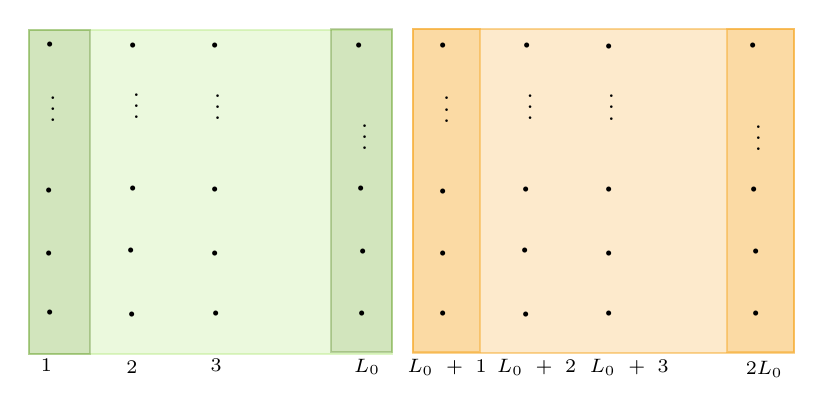
\begin{tikzpicture}[x=0.75pt,y=0.75pt,yscale=-1,xscale=1]
%uncomment if require: \path (0,300); %set diagram left start at 0, and has height of 300

%Shape: Rectangle [id:dp3848625804971728] 
\draw  [color={rgb, 255:red, 184; green, 233; blue, 134 }  ,draw opacity=0.46 ][fill={rgb, 255:red, 184; green, 233; blue, 134 }  ,fill opacity=0.28 ] (234.89,30) -- (410.03,30) -- (410.03,185.94) -- (234.89,185.94) -- cycle ;
%Shape: Rectangle [id:dp9450776254434018] 
\draw  [color={rgb, 255:red, 65; green, 117; blue, 5 }  ,draw opacity=0.29 ][fill={rgb, 255:red, 65; green, 117; blue, 5 }  ,fill opacity=0.15 ] (380.36,29.33) -- (410.03,29.33) -- (410.03,185.28) -- (380.36,185.28) -- cycle ;
%Shape: Rectangle [id:dp43101617233074474] 
\draw  [color={rgb, 255:red, 245; green, 166; blue, 35 }  ,draw opacity=0.47 ][fill={rgb, 255:red, 245; green, 166; blue, 35 }  ,fill opacity=0.23 ] (419.89,29.67) -- (603.69,29.67) -- (603.69,185.61) -- (419.89,185.61) -- cycle ;
%Shape: Rectangle [id:dp31365082950207435] 
\draw  [color={rgb, 255:red, 245; green, 166; blue, 35 }  ,draw opacity=0.46 ][fill={rgb, 255:red, 245; green, 166; blue, 35 }  ,fill opacity=0.24 ] (419.89,29.67) -- (452.36,29.67) -- (452.36,185.28) -- (419.89,185.28) -- cycle ;
%Shape: Rectangle [id:dp8808840272817517] 
\draw  [color={rgb, 255:red, 65; green, 117; blue, 5 }  ,draw opacity=0.29 ][fill={rgb, 255:red, 65; green, 117; blue, 5 }  ,fill opacity=0.15 ] (234.89,30) -- (264.56,30) -- (264.56,185.94) -- (234.89,185.94) -- cycle ;
%Shape: Rectangle [id:dp5267719982198491] 
\draw  [color={rgb, 255:red, 245; green, 166; blue, 35 }  ,draw opacity=0.46 ][fill={rgb, 255:red, 245; green, 166; blue, 35 }  ,fill opacity=0.24 ] (571.22,29.67) -- (603.69,29.67) -- (603.69,185.28) -- (571.22,185.28) -- cycle ;

% Text Node
\draw (240.42,31.05) node [anchor=north west][inner sep=0.75pt]  [font=\LARGE]  {$\cdot $};
% Text Node
\draw (243.37,52.51) node [anchor=north west][inner sep=0.75pt]  [font=\small]  {$\vdots $};
% Text Node
\draw (240.24,101.21) node [anchor=north west][inner sep=0.75pt]  [font=\LARGE]  {$\cdot $};
% Text Node
\draw (240.24,131.49) node [anchor=north west][inner sep=0.75pt]  [font=\LARGE]  {$\cdot $};
% Text Node
\draw (240.28,160.21) node [anchor=north west][inner sep=0.75pt]  [font=\LARGE]  {$\cdot $};
% Text Node
\draw (280.68,31.27) node [anchor=north west][inner sep=0.75pt]  [font=\LARGE]  {$\cdot $};
% Text Node
\draw (283.63,51.3) node [anchor=north west][inner sep=0.75pt]  [font=\small]  {$\vdots $};
% Text Node
\draw (280.36,100.29) node [anchor=north west][inner sep=0.75pt]  [font=\LARGE]  {$\cdot $};
% Text Node
\draw (279.76,130.1) node [anchor=north west][inner sep=0.75pt]  [font=\LARGE]  {$\cdot $};
% Text Node
\draw (280.11,160.87) node [anchor=north west][inner sep=0.75pt]  [font=\LARGE]  {$\cdot $};
% Text Node
\draw (320.17,31.67) node [anchor=north west][inner sep=0.75pt]  [font=\LARGE]  {$\cdot $};
% Text Node
\draw (322.72,51.5) node [anchor=north west][inner sep=0.75pt]  [font=\small]  {$\vdots $};
% Text Node
\draw (320.25,100.69) node [anchor=north west][inner sep=0.75pt]  [font=\LARGE]  {$\cdot $};
% Text Node
\draw (320.25,131.5) node [anchor=north west][inner sep=0.75pt]  [font=\LARGE]  {$\cdot $};
% Text Node
\draw (320.4,160.47) node [anchor=north west][inner sep=0.75pt]  [font=\LARGE]  {$\cdot $};
% Text Node
\draw (354.56,167.68) node [anchor=north west][inner sep=0.75pt]  [font=\small]  {$\dotsc $};
% Text Node
\draw (354.63,137.09) node [anchor=north west][inner sep=0.75pt]  [font=\small]  {$\dotsc $};
% Text Node
\draw (355.03,107.72) node [anchor=north west][inner sep=0.75pt]  [font=\small]  {$\dotsc $};
% Text Node
\draw (355.13,38.18) node [anchor=north west][inner sep=0.75pt]  [font=\small]  {$\dotsc $};
% Text Node
\draw (389.61,31.23) node [anchor=north west][inner sep=0.75pt]  [font=\LARGE]  {$\cdot $};
% Text Node
\draw (393.57,66.1) node [anchor=north west][inner sep=0.75pt]  [font=\small]  {$\vdots $};
% Text Node
\draw (390.23,100.27) node [anchor=north west][inner sep=0.75pt]  [font=\LARGE]  {$\cdot $};
% Text Node
\draw (391.23,130.48) node [anchor=north west][inner sep=0.75pt]  [font=\LARGE]  {$\cdot $};
% Text Node
\draw (390.85,160.43) node [anchor=north west][inner sep=0.75pt]  [font=\LARGE]  {$\cdot $};
% Text Node
\draw (239.25,186.84) node [anchor=north west][inner sep=0.75pt]  [font=\scriptsize]  {$1$};
% Text Node
\draw (280.45,187.75) node [anchor=north west][inner sep=0.75pt]  [font=\scriptsize]  {$2$};
% Text Node
\draw (321.04,186.77) node [anchor=north west][inner sep=0.75pt]  [font=\scriptsize]  {$3$};
% Text Node
\draw (390.19,186.87) node [anchor=north west][inner sep=0.75pt]  [font=\scriptsize]  {$L_{0}$};
% Text Node
\draw (430.09,31.4) node [anchor=north west][inner sep=0.75pt]  [font=\LARGE]  {$\cdot $};
% Text Node
\draw (433.03,52.87) node [anchor=north west][inner sep=0.75pt]  [font=\small]  {$\vdots $};
% Text Node
\draw (429.91,101.57) node [anchor=north west][inner sep=0.75pt]  [font=\LARGE]  {$\cdot $};
% Text Node
\draw (429.91,131.85) node [anchor=north west][inner sep=0.75pt]  [font=\LARGE]  {$\cdot $};
% Text Node
\draw (429.95,160.56) node [anchor=north west][inner sep=0.75pt]  [font=\LARGE]  {$\cdot $};
% Text Node
\draw (470.35,31.62) node [anchor=north west][inner sep=0.75pt]  [font=\LARGE]  {$\cdot $};
% Text Node
\draw (473.3,51.65) node [anchor=north west][inner sep=0.75pt]  [font=\small]  {$\vdots $};
% Text Node
\draw (470.03,100.65) node [anchor=north west][inner sep=0.75pt]  [font=\LARGE]  {$\cdot $};
% Text Node
\draw (469.43,130.45) node [anchor=north west][inner sep=0.75pt]  [font=\LARGE]  {$\cdot $};
% Text Node
\draw (469.78,161.22) node [anchor=north west][inner sep=0.75pt]  [font=\LARGE]  {$\cdot $};
% Text Node
\draw (509.83,32.02) node [anchor=north west][inner sep=0.75pt]  [font=\LARGE]  {$\cdot $};
% Text Node
\draw (512.38,51.85) node [anchor=north west][inner sep=0.75pt]  [font=\small]  {$\vdots $};
% Text Node
\draw (509.91,101.05) node [anchor=north west][inner sep=0.75pt]  [font=\LARGE]  {$\cdot $};
% Text Node
\draw (509.91,131.85) node [anchor=north west][inner sep=0.75pt]  [font=\LARGE]  {$\cdot $};
% Text Node
\draw (510.07,160.82) node [anchor=north west][inner sep=0.75pt]  [font=\LARGE]  {$\cdot $};
% Text Node
\draw (544.23,168.03) node [anchor=north west][inner sep=0.75pt]  [font=\small]  {$\dotsc $};
% Text Node
\draw (544.3,137.45) node [anchor=north west][inner sep=0.75pt]  [font=\small]  {$\dotsc $};
% Text Node
\draw (544.7,108.08) node [anchor=north west][inner sep=0.75pt]  [font=\small]  {$\dotsc $};
% Text Node
\draw (544.79,38.53) node [anchor=north west][inner sep=0.75pt]  [font=\small]  {$\dotsc $};
% Text Node
\draw (579.28,31.58) node [anchor=north west][inner sep=0.75pt]  [font=\LARGE]  {$\cdot $};
% Text Node
\draw (583.24,66.45) node [anchor=north west][inner sep=0.75pt]  [font=\small]  {$\vdots $};
% Text Node
\draw (579.9,100.62) node [anchor=north west][inner sep=0.75pt]  [font=\LARGE]  {$\cdot $};
% Text Node
\draw (580.9,130.83) node [anchor=north west][inner sep=0.75pt]  [font=\LARGE]  {$\cdot $};
% Text Node
\draw (580.52,160.78) node [anchor=north west][inner sep=0.75pt]  [font=\LARGE]  {$\cdot $};
% Text Node
\draw (415.92,187.2) node [anchor=north west][inner sep=0.75pt]  [font=\scriptsize]  {$L_{0} \ +\ 1$};
% Text Node
\draw (459.11,187.1) node [anchor=north west][inner sep=0.75pt]  [font=\scriptsize]  {$L_{0} \ +\ 2$};
% Text Node
\draw (503.71,187.13) node [anchor=north west][inner sep=0.75pt]  [font=\scriptsize]  {$L_{0} \ +\ 3$};
% Text Node
\draw (578.86,188.22) node [anchor=north west][inner sep=0.75pt]  [font=\scriptsize]  {$2L_{0}$};


\end{tikzpicture}

    \caption{Lattice decomposition for the case of periodic boundary conditions. We split the system into two parts, each one has two borders (darker regions). The last time slice $2L_0$ is connected to the first one $1$.}
    \label{fig: fig p bc}
\end{figure}
\\ Using the Schur decomposition \eqref{Schur}, we can write the determinant as:
\begin{equation}
    \det(\mathcal{D}) = \det(B) \det \left[ \begin{pmatrix}
        A & F_2 & \mathbb{0} \\
        F_2' & C & F_3 \\
        \mathbb{0} & F_3' & D
    \end{pmatrix} - \begin{pmatrix}
        F_1' \\
        \mathbb{0} \\
        \mathbb{0} \\
    \end{pmatrix} B^{-1} \begin{pmatrix}
        F_1 & \mathbb{0} & \mathbb{0} \\
    \end{pmatrix}\right]
\end{equation}
If we carry out explicitly the contraction on the last term in the RHS and make use again of the Schur decomposition, we can write:
\begin{equation}\label{decomp pre-M}
    \begin{split}
        \det (\mathcal{D}) &= \det (B) \det \begin{pmatrix}
            A - F_1' B^{-1} F_1 & F_2 & \mathbb{0} \\
            F_2' & C & F_3 \\
            \mathbb{0} & F_3' & D \\
        \end{pmatrix} \\
        &= \det (B) \det (D) \det \begin{pmatrix}
            A - F_1' B^{-1} F_1 & F_2 \\
            F_2' & C - F_3 D^{-1} F_3'
        \end{pmatrix}
    \end{split}
\end{equation}
Given the previous expressions, we have to deal also with the inverse matrices $B^{-1}$ and $D^{-1}$ in order to compute $F_1' B^{-1} F_1$ and $F_3 D^{-1} F_3'$. They can be written in a block-matrix form, and we just need to focus on the $2L_1 \cross 2L_1$ blocks which lie on the corners, namely:
\begin{equation}
    B^{-1} = \begin{pmatrix}
        B_1^{-1} & \dots & B_2^{-1} \\
        \vdots & & \vdots \\
        B_3^{-1} & \dots & B_4^{-1} \\
    \end{pmatrix} \hspace{5mm} D^{-1} = \begin{pmatrix}
        D_1^{-1} & \dots & D_2^{-1} \\
        \vdots & & \vdots \\
        D_3^{-1} & \dots & D_4^{-1} \\
    \end{pmatrix} \
\end{equation}
Notice that it is not necessary to evaluate the full matrices $B^{-1}$ and $D^{-1}$ to find a single block, since we can recursively make use of the relation:
\begin{equation}
    \begin{pmatrix}
        A & B \\
        C & D \\
    \end{pmatrix}^{-1} = \begin{pmatrix}
        \dots & \dots \\
        \dots & (D - CA^{-1}B)^{-1}
    \end{pmatrix} = \begin{pmatrix}
        (A - BD^{-1}C)^{-1} & \dots \\
        \dots & \dots \\
    \end{pmatrix}
\end{equation}
Each block $B_k^{-1}$ and $D_k^{-1}$ can then be decomposed in $L_1 \cross L_1$ blocks:
\begin{equation}
    B_k^{-1} = \begin{pmatrix}
        B_{k,1}^{-1} & B_{k,2}^{-1} \\
        B_{k,3}^{-1} & B_{k,4}^{-1} \\
    \end{pmatrix} \hspace{5mm} D^{-1} = \begin{pmatrix}
        D_{k,1}^{-1} & D_{k,2}^{-1} \\
        D_{k,3}^{-1} & D_{k,4}^{-1} \\
    \end{pmatrix} \
\end{equation}
so that we can evaluate the products $F_1' B^{-1} F_1$ and $F_3 D^{-1} F_3'$:
\begin{equation}
    F_1' B^{-1} F_1 = \begin{pmatrix}
        \mathbb{0} & \Lambda_{1,2} B^{-1}_{1,2} \Bar{\Lambda}_{1,2} & \Lambda_{1,2} B^{-1}_{2,1} \Lambda_{L_0 - 1, L_0} & \mathbb{0} \\
        \mathbb{0} & \mathbb{0} & \mathbb{0} & \mathbb{0} \\
        \mathbb{0} & \mathbb{0} & \mathbb{0} & \mathbb{0} \\
        \mathbb{0} & \Bar{\Lambda}_{L_0 - 1, L_0} B_{3,4}^{-1} \Bar{\Lambda}_{1,2} & \Bar{\Lambda}_{L_0 - 1, L_0} B_{4,3}^{-1} \Bar{\Lambda}_{L_0 - 1,L_0} & \mathbb{0} \\
    \end{pmatrix}
\end{equation}
\begin{equation}
    F_3' D^{-1} F_3 = \begin{pmatrix}
        \mathbb{0} & \mathbb{0} & \mathbb{0} & \mathbb{0} \\
        \Bar{\Lambda}_{2L_0 - 1, 2L_0} D_{4,3}^{-1} \Bar{\Lambda}_{2L_0 - 1, 2L_0}  & \mathbb{0} & \mathbb{0} & \Bar{\Lambda}_{2L_0 - 1, 2L_0} D_{3,4}^{-1} \Bar{\Lambda}_{L_0 + 1, L_0 + 2} \\
        \Lambda_{L_0 + 1, L_0 + 2} D^{-1}_{2,1} \Lambda_{2L_0 - 1, 2L_0} & \mathbb{0} & \mathbb{0} & \Lambda_{L_0 + 1, L_0 + 2} D^{-1}_{1,2} \Bar{\Lambda}_{L_0 + 1, L_0 + 2} \\
        \mathbb{0} & \mathbb{0} & \mathbb{0} & \mathbb{0} \\
    \end{pmatrix}
\end{equation}
Given the previous definitions, it follows immediately that:
\begin{equation}
\begin{split}
    &A - F_1' B^{-1} F_1 = \begin{pmatrix}
        X_1 & \Tilde{Y}_1 & \Tilde{\Lambda}_{1, L_0} & \mathbb{0} \\
        Y_1 & X_1 & \mathbb{0} & \mathbb{0} \\
        \mathbb{0} & \mathbb{0} & X_{L_0} & Y_{L_0} \\
        \mathbb{0} & \Tilde{\Lambda}_{L_0, 1} & \Tilde{Y}_{L_0} & X_{L_0} \\
    \end{pmatrix} \\ &C - F_3' D^{-1} F_3 = \begin{pmatrix}
        X_{2L_0} & Y_{2L_0} & \mathbb{0} & \mathbb{0} \\
        \Tilde{Y}_{2L_0} & X_{2L_0} & \mathbb{0} & \Tilde{\Lambda}_{2L_0, L_0 + 1} \\
        \Tilde{\Lambda}_{L_0 + 1, 2L_0} & \mathbb{0} & X_{L_0 + 1} & \Tilde{Y}_{L_0 + 1} \\
        \mathbb{0} & \mathbb{0} & Y_{L_0 + 1} & X_{L_0 + 1} \\
    \end{pmatrix}
    \end{split}
\end{equation}
where we introduced:
\begin{equation}
    \begin{split}
       & \Tilde{Y}_1 = Y_1 - \Lambda_{1,2} B^{-1}_{1,2} \Bar{\Lambda}_{1,2} \\
       & \Tilde{Y}_{L_0} = Y_{L_0} - \Bar{\Lambda}_{L_0 - 1,L_0} B^{-1}_{4,3} \Lambda_{L_0 - 1, L_0} \\
       & \Tilde{Y}_{L_0 + 1} = Y_{L_0 + 1} - \Lambda_{L_0 + 1,L_0 + 2} D^{-1}_{1,2} \Bar{\Lambda}_{L_0 + 1,L_0 + 2} \\
       & \Tilde{Y}_{2L_0} = Y_{2L_0} - \Bar{\Lambda}_{2L_0 - 1,2L_0} D^{-1}_{4,3} \Lambda_{2L_0 - 1, 2L_0} \\
       & \Tilde{\Lambda}_{1, L_0} = - \Lambda_{1,2} B^{-1}_{2,1} \Lambda_{L_0 - 1, L_0} \\
       & \Tilde{\Lambda}_{L_0, 1} = - \Bar{\Lambda}_{L_0 - 1, L_0} B_{3,4}^{-1} \Bar{\Lambda}_{1,2} \\
       & \Tilde{\Lambda}_{2L_0, L_0 + 1} = - \Bar{\Lambda}_{2L_0 - 1, 2L_0} D_{3,4}^{-1} \Bar{\Lambda}_{L_0 + 1, L_0 + 2} \\
       & \Tilde{\Lambda}_{L_0 + 1, L_0 + 2} = -  \Lambda_{L_0 + 1, L_0 + 2} D^{-1}_{2,1} \Lambda_{2L_0 - 1, 2L_0}
    \end{split}
\end{equation}
Hence we can rewrite the last matrix on the RHS of \eqref{decomp pre-M} as:
\begin{equation}
    \mathcal{M} = \begin{pmatrix}
         X_1 & \Tilde{Y}_1 & \Tilde{\Lambda}_{1, L_0} & \mathbb{0}  & \mathbb{0}  & \mathbb{0} & \mathbb{0}  \\
        Y_1 & X_1 & \mathbb{0} & \mathbb{0}  & \mathbb{0} & \Bar{\Lambda}_{2L_0, 1} & \mathbb{0}  & \mathbb{0} \\
        \mathbb{0} & \mathbb{0} & X_{L_0} & Y_{L_0}  & \mathbb{0}  & \mathbb{0} & \Lambda_{L_0, L_0 + 1}  & \mathbb{0} \\
        \mathbb{0} & \Tilde{\Lambda}_{L_0, 1} & \Tilde{Y}_{L_0} & X_{L_0}  & \mathbb{0}  & \mathbb{0} & \mathbb{0}  & \mathbb{0} \\
        \Lambda_{2L_0, 1} & \mathbb{0} & \mathbb{0} & \mathbb{0} & X_{2L_0} & Y_{2L_0} & \mathbb{0} & \mathbb{0} \\
        \mathbb{0} & \mathbb{0} & \mathbb{0} & \mathbb{0} & \Tilde{Y}_{2L_0} & X_{2L_0} & \mathbb{0} & \Tilde{\Lambda}_{2L_0, L_0 + 1} \\
        \mathbb{0} & \mathbb{0} & \mathbb{0} & \mathbb{0} & \Tilde{\Lambda}_{L_0 + 1, 2L_0} & \mathbb{0} & X_{L_0 + 1} & \Tilde{Y}_{L_0 + 1} \\
        \mathbb{0} & \mathbb{0} & \mathbb{0} & \Bar{\Lambda}_{L_0, L_0 + 1} & \mathbb{0} & \mathbb{0} & Y_{L_0 + 1} & X_{L_0 + 1} \\
    \end{pmatrix}
\end{equation}
and \eqref{decomp pre-M} becomes:
\begin{equation}
    \det(\mathcal{D}) = \det(B) \det(D) \det(\mathcal{M})
\end{equation}
It is now convenient to perform some rotations which leave $\det(\mathcal{M})$ invariant: by swapping rows and columns $(2 \leftrightarrow 4)$ and $(6 \leftrightarrow 8)$ and by recasting the resulting blocks similarly to what we did in \eqref{rot}, we get the matrix:
\begin{equation}
    \mathcal{M} = \begin{pmatrix}
         \mathbb{0} & \mathbb{0} & \Tilde{\Lambda}_{1, L_0} & \Tilde{Y}_1 & X_1  \mathbb{0}  & \mathbb{0} & \mathbb{0}  \\
        \mathbb{0} & \mathbb{0} & \Tilde{Y}_{L_0} & \Tilde{\Lambda}_{L_0, 1}  & \mathbb{0} & X_{L_0} & \mathbb{0}  & \mathbb{0} \\
        \Tilde{\Lambda}_{L_0 + 1, 2L_0} & \Tilde{Y}_{L_0 + 1} & \mathbb{0} & \mathbb{0}  & \mathbb{0} & \mathbb{0} & X_{L_0 + 1}  & \mathbb{0} \\
        \Tilde{Y}_{2L_0} &  \Tilde{\Lambda}_{2L_0, L_0 + 1} & \mathbb{0} & \mathbb{0} & \mathbb{0} & \mathbb{0} & \mathbb{0} & X_{2L_0} \\
        X_{2L_0} & \mathbb{0} & \mathbb{0} & \mathbb{0} & \Lambda_{2L_0, 1} & \mathbb{0} & \mathbb{0} & \mathbb{0} \\
        \mathbb{0} & X_{L_0 + 1} & \mathbb{0} & \mathbb{0} & \mathbb{0} & \Bar{\Lambda}_{L_0, L_0 + 1} & Y_{L_0 + 1} & \mathbb{0} \\
        \mathbb{0} & \mathbb{0} & X_{L_0} & \mathbb{0} & \mathbb{0} & Y_{L_0} & \Lambda_{L_0, L_0 + 1} & \mathbb{0} \\
        \mathbb{0} & \mathbb{0} & \mathbb{0} & X_1 & Y_1 & \mathbb{0} & \mathbb{0} & \Bar{\Lambda}_{2L_0, 1} \\
    \end{pmatrix}
\end{equation}
and since we will need to refer to some portions of this matrix, we can label its blocks as:
\begin{equation}
    \mathcal{M} = \begin{pmatrix}
        \mathcal{M}_{1,1} &  \mathcal{M}_{1,2} \\ 
         \mathcal{M}_{2,1} &  \mathcal{M}_{2,2} \\
    \end{pmatrix} \hspace{2mm} \Dot{Y}_{1, L_0} = \begin{pmatrix}
        \Tilde{\Lambda}_{1, L_0} & \Tilde{Y}_1 \\
        \Tilde{Y}_{L_0} & \Tilde{\Lambda}_{L_0, 1} \\
    \end{pmatrix} \hspace{2mm} \Dot{Y}_{L_0 + 1, 2L_0} = \begin{pmatrix}
        \Tilde{\Lambda}_{L_0 + 1, 2L_0} & \Tilde{Y}_{L_0 + 1} \\
        \Tilde{Y}_{2L_0} & \Tilde{\Lambda}_{2L_0, L_0 + 1} \\
    \end{pmatrix}
\end{equation}
Now we can use the usual Schur decomposition to write:
\begin{equation}\label{det M pbc}
    \det(\mathcal{M}) = \det(\Dot{Y}_{1, L_0}) \det(\Dot{Y}_{L_0 + 1, 2L_0}) \det\left[\mathcal{M}_{2,2} - \mathcal{M}_{2,1} \begin{pmatrix}
        \mathbb{0} & (\Dot{Y}_{L_0 + 1, 2L_0})^{-1} \\
        (\Dot{Y}_{1, L_0})^{-1} & \mathbb{0} \\
    \end{pmatrix} \mathcal{M}_{1,2} \right] 
\end{equation}
The last determinant in the RHS needs to be factorized, hence it is useful to define the matrix:
\begin{equation}
    \Tilde{d} = \begin{pmatrix}
        \Lambda_{2L_0, 1} & \mathbb{0} & (\hat{Y}_{L_0 + 1, 2L_0})_{1,1} & (\hat{Y}_{L_0 + 1, 2L_0})_{1,2} \\
        \mathbb{0} & \Bar{\Lambda}_{L_0, L_0 + 1} & (\hat{Y}_{L_0 + 1, 2L_0})_{2,1} & (\hat{Y}_{L_0 + 1, 2L_0})_{2,2} \\
        (\hat{Y}_{1, L_0})_{1,1} & (\hat{Y}_{1, L_0})_{1,2} & \Lambda_{L_0, L_0 + 1} & \mathbb{0} \\
        (\hat{Y}_{1, L_0})_{2,1} & (\hat{Y}_{1, L_0})_{2,2} & \mathbb{0} & \Bar{\Lambda}_{2L_0, 1}
    \end{pmatrix}
\end{equation}
where $(\hat{Y}_{\dots})_{i, j}$ denote the blocks of the following matrices of dimensions $2L_1 \cross 2L_1$:
\begin{equation}
    \begin{split}
        & \hat{Y}_{1, L_0} = \begin{pmatrix}
            \mathbb{0} & Y_{L_0} \\
            Y_1 & \mathbb{0} \\
        \end{pmatrix} - \begin{pmatrix}
            X_{L_0} & \mathbb{0} \\ 
            \mathbb{0} & X_{1} \\
        \end{pmatrix} (\Dot{Y}_{1, L_0})^{-1} \begin{pmatrix}
            X_1 & \mathbb{0} \\
            \mathbb{0} & X_{L_0} \\
        \end{pmatrix} \\
        & \hat{Y}_{L_0 + 1, 2L_0} = \begin{pmatrix}
            \mathbb{0} & Y_{2L_0} \\
            Y_{L_0 + 1} & \mathbb{0} \\
        \end{pmatrix} - \begin{pmatrix}
            X_{2L_0} & \mathbb{0} \\ 
            \mathbb{0} & X_{L_0 + 1} \\
        \end{pmatrix} (\Dot{Y}_{L_0 + 1, 2L_0})^{-1} \begin{pmatrix}
            X_{L_0 + 1} & \mathbb{0} \\
            \mathbb{0} & X_{2L_0} \\
        \end{pmatrix}
    \end{split}
\end{equation}
It is now convenient to perform a rotation that leaves the determinant of $\Tilde{d}$ invariant (hence we will still call the result of the rotation $\Tilde{d})$:
\begin{equation}
\begin{split}
        \Tilde{d} \to & \begin{pmatrix}
            \mathbb{0} & \mathbb{0} & \mathbb{0} & \mathbb{1} \\
            \mathbb{0} & \mathbb{0} & \mathbb{1} & \mathbb{0} \\
            \mathbb{1} & \mathbb{0} & \mathbb{0} & \mathbb{0} \\
            \mathbb{0} & \mathbb{1} & \mathbb{0} & \mathbb{0} \\
        \end{pmatrix} \Tilde{d} \begin{pmatrix}
            \mathbb{0} & \mathbb{0} & \mathbb{1} & \mathbb{0} \\
            \mathbb{0} & \mathbb{0} & \mathbb{0} & \mathbb{1} \\
            \mathbb{0} & \mathbb{1} & \mathbb{0} & \mathbb{0} \\
            \mathbb{1} & \mathbb{0} & \mathbb{0} & \mathbb{0} \\
        \end{pmatrix} = \\ &= \begin{pmatrix}
        \Bar{\Lambda}_{2L_0, 1} & \mathbb{0} & (\hat{Y}'_{1, L_0})_{1,1} & (\hat{Y}'_{1, L_0})_{1,2} \\
        \mathbb{0} & \Lambda_{L_0, L_0 + 1} & (\hat{Y}'_{1, L_0})_{2,1} & (\hat{Y}'_{1, L_0})_{2,2} \\
        (\hat{Y}'_{L_0 + 1, 2L_0})_{1,1} & (\hat{Y}'_{L_0 + 1, 2L_0})_{1,2} & \Lambda_{2L_0, 1} & \mathbb{0} \\
        (\hat{Y}'_{L_0 + 1, 2L_0})_{2,1} & (\hat{Y}'_{L_0 + 1, 2L_0})_{2,2} & \mathbb{0} & \Bar{\Lambda}_{L_0, L_0 + 1}
    \end{pmatrix}
    \end{split}
\end{equation}
Where now the $\hat{Y}'$ matrices are given by:
\begin{equation}
    \Hat{Y}'_{1, L_0} = \begin{pmatrix}
        Y_{1} & \mathbb{0} \\
        \mathbb{0} & Y_{L_0}
    \end{pmatrix} - \begin{pmatrix}
        \mathbb{0} & X_1 \\
        X_{L_0} &  \mathbb{0} \\
    \end{pmatrix} (\Dot{Y}_{1, L_0})^{-1} \begin{pmatrix}
        X_1 & \mathbb{0} \\
        \mathbb{0} & X_{L_0} \\
    \end{pmatrix}
\end{equation}
\begin{equation}
    \Hat{Y}'_{L_0 + 1, 2L_0} = \begin{pmatrix}
        Y_{2L_0} & \mathbb{0} \\
        \mathbb{0} & Y_{L_0 + 1}
    \end{pmatrix} - \begin{pmatrix}
        X_{2L_0} & \mathbb{0} \\
        \mathbb{0} & X_{L_0 + 1} \\
    \end{pmatrix} (\Dot{Y}_{L_0 + 1, 2L_0})^{-1} \begin{pmatrix}
        \mathbb{0} & X_{L_0 + 1} \\
        X_{2L_0} & \mathbb{0}
    \end{pmatrix}
\end{equation}
Analogously to the case of open boundary conditions, we can define the square roots of $\Lambda_{i,j}$:
\begin{equation}
    \lambda_{L_0, L_0 + 1} = \sqrt{\Lambda_{L_0, L_0 + 1}} \hspace{4mm} \Bar{\lambda}_{2L_0, 1} = \sqrt{\Bar{\Lambda}_{2L_0, 1}} \longrightarrow \lambda_i \Bar{\lambda}_i = \mathbb{1}
\end{equation}
so that we can implement a transformation which leaves $\det(\Tilde{d})$ invariant:
\begin{equation}
        \begin{pmatrix}
        i\lambda_{2L_0, 1} & \mathbb{0} & \mathbb{0} & \mathbb{0} \\
        \mathbb{0} & \Bar{\lambda}_{L_0, L_0 + 1} & \mathbb{0} & \mathbb{0} \\
        \mathbb{0} & \mathbb{0} & -i\Bar{\lambda}_{2L_0, 1} & \mathbb{0} \\
        \mathbb{0} & \mathbb{0} & \mathbb{0} & \lambda_{L_0, L_0 + 1} \\
    \end{pmatrix} \Tilde{d} \begin{pmatrix}
        -i\lambda_{2L_0, 1} & \mathbb{0} & \mathbb{0} & \mathbb{0} \\
        \mathbb{0} & \bar{\lambda}_{L_0, L_0 + 1} & \mathbb{0} & \mathbb{0} \\
        \mathbb{0} & \mathbb{0} & i\Bar{\lambda}_{2L_0, 1} & \mathbb{0} \\
        \mathbb{0} & \mathbb{0} & \mathbb{0} & \lambda_{L_0, L_0 + 1} \\
    \end{pmatrix}
\end{equation}
For the sake of clarity, as the determinant does not change, we can still call the result $\Tilde{d}$:
\begin{equation}\label{tilde d}
    \Tilde{d} = \begin{pmatrix}
        \mathbb{1} & \accentset{\ast}{Y}_{1, L_0} \\
        \accentset{\ast}{Y}_{L_0 + 1, 2L_0} & \mathbb{1} \\
    \end{pmatrix}
\end{equation}
where $\accentset{\ast}{Y}_{1, L_0}$ and $\accentset{\ast}{Y}_{L_0 + 1, 2L_0}$ are anti-Hermitian matrices defined by:
\begin{equation}
    \begin{split}
        & \accentset{\ast}{Y}_{1, L_0} = \begin{pmatrix}
            i\lambda_{2L_0, 1} & \mathbb{0} \\
            \mathbb{0} & \bar{\lambda}_{L_0, L_0 + 1}
        \end{pmatrix} \hat{Y}'_{1, L_0} \begin{pmatrix}
            i\Bar{\lambda}_{2L_0, 1} & \mathbb{0} \\
            \mathbb{0} & \lambda_{L_0, L_0 + 1}
        \end{pmatrix} \\
        & \accentset{\ast}{Y}_{L_0 + 1, 2L_0} = \begin{pmatrix}
            -i\Bar{\lambda}_{2L_0, 1} & \mathbb{0} \\
            \mathbb{0} & \lambda_{L_0, L_0 + 1}
        \end{pmatrix} \hat{Y}'_{L_0 + 1, 2L_0} \begin{pmatrix}
            -i\lambda_{2L_0, 1} & \mathbb{0} \\
            \mathbb{0} & \bar{\lambda}_{2L_0, 1}
        \end{pmatrix}
    \end{split}
\end{equation}
Therefore by putting \eqref{decomp pre-M} and \eqref{det M pbc} together, the determinant of the Dirac operator can be written as:
\begin{equation}\label{det D pbc}
    \det(\mathcal{D}) = \det(\mathcal{D}_{2, L_0 - 1}) \det(\mathcal{D}_{L_0 + 2, 2L_0 - 1}) \det(\Dot{Y}_{1, L_0}) \det(\Dot{Y}_{L_0 + 1, 2L_0}) \det(\Tilde{d})
\end{equation}
and the factorization is complete for all the terms but $\det(\Tilde{d})$. Notice that the procedure for periodic boundary conditions follows closely what we have already seen for open boundary conditions in Section \ref{OpenBC}, but since in this case the domains $[1, L_0]$ and $[L_0 + 1, 2L_0]$ have two borders rather than one, the dimensionality of $\Tilde{d}$ is doubled with respect to the previous study.
Keeping in mind this difference, we can introduce analogous bosonic variables $\{\sigma_i\}_{i = 1\dots 4L_1}$ and reproduce the same steps as in \eqref{Begin Pfaffian}-\eqref{Final Pfaffian}. 
One can show that, constructing the real matrices:
\begin{equation}\label{Initial SA SB}
   \accentset{\ast}{K}_{L_0} = \frac{1}{2}\begin{pmatrix}
        \accentset{\ast}{Y}_{L_0} - \accentset{\ast}{Y}_{1, L_0}^T & -i (\accentset{\ast}{Y}_{1, L_0} + \accentset{\ast}{Y}_{1, L_0}^T) \\
        \\
        i(\accentset{\ast}{Y}_{1, L_0} + \accentset{\ast}{Y}_{1, L_0}^T) & \accentset{\ast}{Y}_{1, L_0} - \accentset{\ast}{Y}_{L_0}^T \\
    \end{pmatrix}
\end{equation}
\begin{equation}
   \accentset{\ast}K_{L_0 + 1} = \frac{1}{2}\begin{pmatrix}
        -\accentset{\ast}{Y}_{L_0 + 1} + \accentset{\ast}{Y}_{L_0 + 1, 2L_0}^T & i (\accentset{\ast}{Y}_{L_0 + 1, 2L_0} + \accentset{\ast}{Y}_{L_0 + 1, 2L_0}^T) \\
        \\
        -i(\accentset{\ast}{Y}_{L_0 + 1, 2L_0} + \accentset{\ast}{Y}_{L_0 + 1, 2L_0}^T) & - \accentset{\ast}{Y}_{L_0 + 1, 2L_0} + \accentset{\ast}{Y}_{L_0 + 1, 2L_0}^T \\
    \end{pmatrix}
\end{equation}
\begin{equation}
    \accentset{\ast}{J}(\sigma) = \begin{pmatrix}
        \sigma_1 & \\
        & \ddots & \\
        \\
        & & & \sigma_{4L_1} \\
    \end{pmatrix}\begin{pmatrix}
        0 & 1 & 1 & \dots \\
        -1 & 0 & 1  \\
        -1 & - 1 & \ddots & \\
        \vdots & \\
        & & & & 0 \\
    \end{pmatrix}
    \begin{pmatrix}
        \sigma_1 & \\
        & \ddots & \\
        \\
        & & & \sigma_{4L_1} \\
    \end{pmatrix}
\end{equation}
the determinant $\det(\Tilde{d})$ can be written as:
\begin{equation}\label{det d tilde pbc}
\begin{split}
\det (\Tilde{d}) = \int \mathcal{D}[\sigma] \left[\mathcal{D}[\chi_A] e^{-\frac{1}{2}\chi_A^T S_A \chi_A} \right] \left[\mathcal{D}[\chi_B] e^{-\frac{1}{2}\chi_B^T S_B \chi_B} \right] \\
        \rightarrow \det(\Tilde{d}) = \int \mathcal{D}[\sigma] \textrm{Pf}(S_A)\textrm{Pf}(S_B) \hspace{25mm}
\end{split}
\end{equation}
where:
\begin{equation}\label{final SA SB}
    S_A = \accentset{\ast}{K}_{L_0} + \accentset{\ast}{J}(\sigma) \hspace{5 mm} S_B = \accentset{\ast}{K}_{L_0 + 1} - \accentset{\ast}{J}(\sigma)
\end{equation}
and since $S_A$ and $S_B$ are real skew-symmetric matrices, their Pfaffian is also real.
\\ Putting \eqref{det D pbc} and \eqref{det d tilde pbc} together:
\begin{equation}
    \det(\mathcal{D}) = \int \mathcal{D}[\sigma] \textrm{Pf}(S_A)\textrm{Pf}(S_B) \det(\mathcal{D}_{1, L_0 - 1}) \det(\mathcal{D}_{L_0 + 1, 2L_0}) \det(\Tilde{Y}_{L_0})  \det(\Tilde{Y}_{L_0 + 1})
\end{equation}
we achieve a full factorization of the fermionic determinant.

\section{Numerical test}
In this section we will give some numerical evidence of the complete factorization of the fermionic determinant.
\\ We performed the following tests embedding anti-periodic boundary conditions in the time direction, since these were the boundary conditions held throughout all the previous simulations, and they can be achieved by following the prescription described in the section for periodic boundary conditions and by adding an additive minus sign to the definitions of the matrices $\Lambda_{2L_0, 1}$ and $\Bar{\Lambda}_{2L_0, 1}$. Taken into account this small modification, we want to check the validity of the relation:
\begin{equation}\label{fact pf}
\begin{split}
\det (\Tilde{d}) = \int \mathcal{D}[\sigma] \left[\mathcal{D}[\chi_A] e^{-\frac{1}{2}\chi_A^T S_A \chi_A} \right] \left[\mathcal{D}[\chi_B] e^{-\frac{1}{2}\chi_B^T S_B \chi_B} \right] \\
        \rightarrow \det(\Tilde{d}) = \int \mathcal{D}[\sigma] \textrm{Pf}(S_A)\textrm{Pf}(S_B) \hspace{25mm}
\end{split}
\end{equation}
where the definition of $\Tilde{d}$ is given in \eqref{tilde d}, while $S_A$ and $S_B$ are defined in \eqref{Initial SA SB}-\eqref{final SA SB}.
\\ As we mentioned in the previous section, we can choose different kind of variables for the bosonic fields $\{\sigma\}_{i = 1, \dots, 4L_1}$, for instance Ising variables $\sigma = \{1, -1\}$ and Gaussianly distributed variables. Since the first ones take value over a finite set of numbers, we can perform an explicit computation of the integral over bosonic fields, which in turn becomes a summation of $2^{4L_1}$ terms.
\\ We performed this computation for lattices of extension $4 \times 8$, $4 \times 16$ and $6 \times 16$ with $\beta = 2$ and $m_0 = 0.2$, and in each case the relation \eqref{fact pf} was satisfied exactly. This proves numerically that with the procedure presented in this document, we can achieve a complete factorization of the fermionic determinant, and in literature this is the first prescription where such a result is obtained. 
Notice that the numerical computation of the Pfaffian was carried out using the MATLAB library presented in \cite{Wimmer_2012}. 
\\ We can give a differ insight of the goodness of our factorization procedure by showing some results where Gaussianly distributed variables were embedded as bosonic fields $\sigma$. Namely, we can introduce an ensemble of $N_{\textrm{sources}}$ sets of variables distributed accordingly to a Gaussian $\mathcal{N}(0,1)$, i.e. each set contains the $4L_1$ bosonic fields $\sigma$. Given a gauge configuration extrapolated from our code, we can use this ensemble to offer a stochastic estimation of the integration over $\sigma$ in the RHS of \eqref{fact pf}, by evaluating the Pfaffians over each set of bosonic fields $\{\sigma\}_{i = 1, \dots, 4L_1}^{n = 1, \dots, N_{\textrm{sources}}}$ and taking the average. 
\\ In Figure \eqref{fig: pfaf 4x8}-\eqref{fig: pfaf 6x16} we compare these estimations, computed with an increasing volume of sources, with the exact computation of $\det(\Tilde{d})$, represented by a horizontal line in each plot.
\begin{figure}
    \centering
    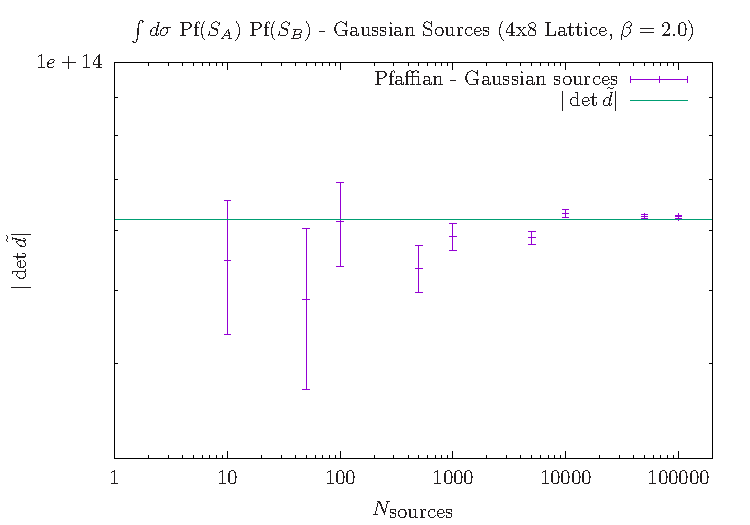
\includegraphics[width=0.8\linewidth]{images/pfaffian4x8.pdf}
    \caption{Numerical test for relation \eqref{fact pf}. This computation was performed on a $4 \times 8$ lattice with $\beta = 2$ and $m_0 = 0.2$.
    The number of sources ranges from 10 to 100000, and the horizontal line represents the value of $\det(\Tilde{d})$.}
    \label{fig: pfaf 4x8}
\end{figure}
\begin{figure}
    \centering
    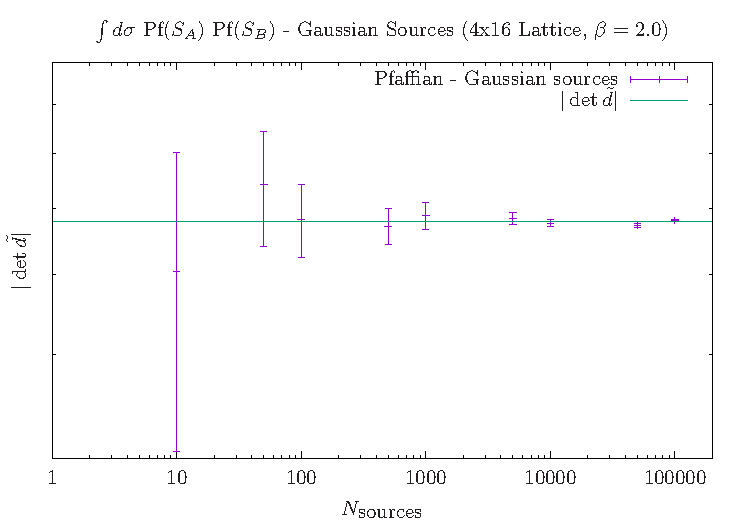
\includegraphics[width=0.8\linewidth]{images/pfaffian4x16.pdf}
    \caption{Numerical test for relation \eqref{fact pf}. This computation was performed on a $4 \times 16$ lattice with $\beta = 2$ and $m_0 = 0.2$.
    The number of sources ranges from 10 to 100000, and the horizontal line represents the value of $\det(\Tilde{d})$.}
    \label{fig: pfaf 4x16}
\end{figure}
\begin{figure}
    \centering
    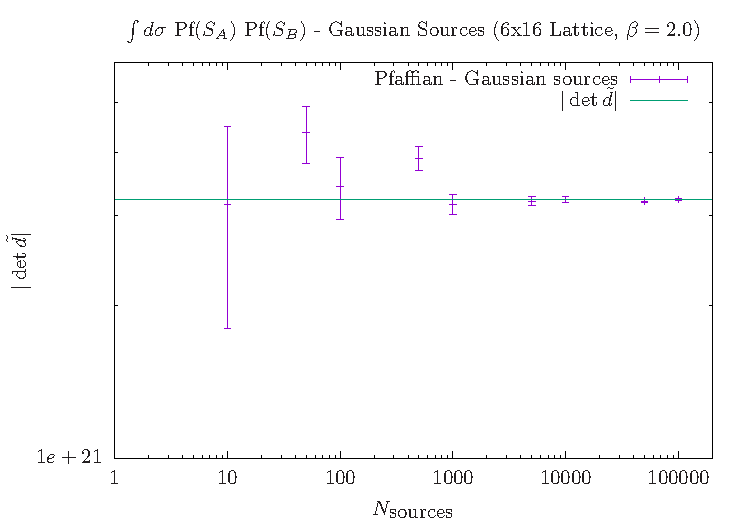
\includegraphics[width=0.8\linewidth]{images/pfaffian6x16.pdf}
    \caption{Numerical test for relation \eqref{fact pf}. This computation was performed on a $6 \times 16$ lattice with $\beta = 2$ and $m_0 = 0.2$.
    The number of sources ranges from 10 to 100000, and the horizontal line represents the value of $\det(\Tilde{d})$.}
    \label{fig: pfaf 6x16}
\end{figure}
Although we performed this tests on small lattices, it is clear that, given a sufficiently large amount of sources, the accordance between $\det(\Tilde{d})$ and the computation employing the Pfaffians is absolutely satisfying also with this stochastic estimation.
\\ These results confirm the goodness of our factorization procedure, which we consider extremely interesting as it allows for a complete separation of the system dynamics and could guarantee a natural factorization of the observables. Indeed the factorization of fermionic observables is the next goal of this research line, as it will allow us to perform deeper analysis about this factorization prescription, in the hope that it actually brings significant improvement in the state of art of lattice computations.